\documentclass[twoside]{book}

% Packages required by doxygen
\usepackage{calc}
\usepackage{doxygen}
\usepackage{graphicx}
\usepackage[utf8]{inputenc}
\usepackage{makeidx}
\usepackage{multicol}
\usepackage{multirow}
\usepackage{textcomp}
\usepackage[table]{xcolor}

% Font selection
\usepackage[T1]{fontenc}
\usepackage{mathptmx}
\usepackage[scaled=.90]{helvet}
\usepackage{courier}
\usepackage{amssymb}
\usepackage{sectsty}
\renewcommand{\familydefault}{\sfdefault}
\allsectionsfont{%
  \fontseries{bc}\selectfont%
  \color{darkgray}%
}
\renewcommand{\DoxyLabelFont}{%
  \fontseries{bc}\selectfont%
  \color{darkgray}%
}

% Page & text layout
\usepackage{geometry}
\geometry{%
  a4paper,%
  top=2.5cm,%
  bottom=2.5cm,%
  left=2.5cm,%
  right=2.5cm%
}
\tolerance=750
\hfuzz=15pt
\hbadness=750
\setlength{\emergencystretch}{15pt}
\setlength{\parindent}{0cm}
\setlength{\parskip}{0.2cm}
\makeatletter
\renewcommand{\paragraph}{%
  \@startsection{paragraph}{4}{0ex}{-1.0ex}{1.0ex}{%
    \normalfont\normalsize\bfseries\SS@parafont%
  }%
}
\renewcommand{\subparagraph}{%
  \@startsection{subparagraph}{5}{0ex}{-1.0ex}{1.0ex}{%
    \normalfont\normalsize\bfseries\SS@subparafont%
  }%
}
\makeatother

% Headers & footers
\usepackage{fancyhdr}
\pagestyle{fancyplain}
\fancyhead[LE]{\fancyplain{}{\bfseries\thepage}}
\fancyhead[CE]{\fancyplain{}{}}
\fancyhead[RE]{\fancyplain{}{\bfseries\leftmark}}
\fancyhead[LO]{\fancyplain{}{\bfseries\rightmark}}
\fancyhead[CO]{\fancyplain{}{}}
\fancyhead[RO]{\fancyplain{}{\bfseries\thepage}}
\fancyfoot[LE]{\fancyplain{}{}}
\fancyfoot[CE]{\fancyplain{}{}}
\fancyfoot[RE]{\fancyplain{}{\bfseries\scriptsize Generated on Tue Dec 17 2013 20\-:05\-:04 for Pro\-Scan\-Mobile+ by Doxygen }}
\fancyfoot[LO]{\fancyplain{}{\bfseries\scriptsize Generated on Tue Dec 17 2013 20\-:05\-:04 for Pro\-Scan\-Mobile+ by Doxygen }}
\fancyfoot[CO]{\fancyplain{}{}}
\fancyfoot[RO]{\fancyplain{}{}}
\renewcommand{\footrulewidth}{0.4pt}
\renewcommand{\chaptermark}[1]{%
  \markboth{#1}{}%
}
\renewcommand{\sectionmark}[1]{%
  \markright{\thesection\ #1}%
}

% Indices & bibliography
\usepackage{natbib}
\usepackage[titles]{tocloft}
\setcounter{tocdepth}{3}
\setcounter{secnumdepth}{5}
\makeindex

% Hyperlinks (required, but should be loaded last)
\usepackage{ifpdf}
\ifpdf
  \usepackage[pdftex,pagebackref=true]{hyperref}
\else
  \usepackage[ps2pdf,pagebackref=true]{hyperref}
\fi
\hypersetup{%
  colorlinks=true,%
  linkcolor=blue,%
  citecolor=blue,%
  unicode%
}

% Custom commands
\newcommand{\clearemptydoublepage}{%
  \newpage{\pagestyle{empty}\cleardoublepage}%
}


%===== C O N T E N T S =====

\begin{document}

% Titlepage & ToC
\hypersetup{pageanchor=false}
\pagenumbering{roman}
\begin{titlepage}
\vspace*{7cm}
\begin{center}%
{\Large Pro\-Scan\-Mobile+ }\\
\vspace*{1cm}
{\large Generated by Doxygen 1.8.5}\\
\vspace*{0.5cm}
{\small Tue Dec 17 2013 20:05:04}\\
\end{center}
\end{titlepage}
\clearemptydoublepage
\tableofcontents
\clearemptydoublepage
\pagenumbering{arabic}
\hypersetup{pageanchor=true}

%--- Begin generated contents ---
\chapter{Namespace Index}
\section{Packages}
Here are the packages with brief descriptions (if available)\-:\begin{DoxyCompactList}
\item\contentsline{section}{\hyperlink{namespace_pro_scan_mobile}{Pro\-Scan\-Mobile} }{\pageref{namespace_pro_scan_mobile}}{}
\end{DoxyCompactList}

\chapter{Hierarchical Index}
\section{Class Hierarchy}
This inheritance list is sorted roughly, but not completely, alphabetically\-:\begin{DoxyCompactList}
\item \contentsline{section}{Pro\-Scan\-Mobile.\-Application}{\pageref{class_pro_scan_mobile_1_1_application}}{}
\item \contentsline{section}{Pro\-Scan\-Mobile.\-Encryption}{\pageref{class_pro_scan_mobile_1_1_encryption}}{}
\item \contentsline{section}{Pro\-Scan\-Mobile.\-Network\-Connection}{\pageref{class_pro_scan_mobile_1_1_network_connection}}{}
\item \contentsline{section}{Pro\-Scan\-Mobile.\-Read\-Write\-Buffer}{\pageref{class_pro_scan_mobile_1_1_read_write_buffer}}{}
\item \contentsline{section}{Pro\-Scan\-Mobile.\-Rec\-Table\-Item}{\pageref{class_pro_scan_mobile_1_1_rec_table_item}}{}
\item \contentsline{section}{Pro\-Scan\-Mobile.\-Scanner\-Audio}{\pageref{class_pro_scan_mobile_1_1_scanner_audio}}{}
\item \contentsline{section}{Pro\-Scan\-Mobile.\-Scanner\-Screen}{\pageref{class_pro_scan_mobile_1_1_scanner_screen}}{}
\item \contentsline{section}{Pro\-Scan\-Mobile.\-vc\-Options\-Screen.\-Server\-Details}{\pageref{class_pro_scan_mobile_1_1vc_options_screen_1_1_server_details}}{}
\item \contentsline{section}{Pro\-Scan\-Mobile.\-vc\-Options\-Screen.\-Servers}{\pageref{class_pro_scan_mobile_1_1vc_options_screen_1_1_servers}}{}
\item \contentsline{section}{Pro\-Scan\-Mobile.\-vc\-Options\-Screen.\-Settings}{\pageref{class_pro_scan_mobile_1_1vc_options_screen_1_1_settings}}{}
\item \contentsline{section}{Pro\-Scan\-Mobile.\-vc\-Options\-Screen.\-Settings\-Details}{\pageref{class_pro_scan_mobile_1_1vc_options_screen_1_1_settings_details}}{}
\item \contentsline{section}{Pro\-Scan\-Mobile.\-Network\-Connection.\-State\-Object}{\pageref{class_pro_scan_mobile_1_1_network_connection_1_1_state_object}}{}
\item \contentsline{section}{Pro\-Scan\-Mobile.\-Streaming\-Playback\-V2}{\pageref{class_pro_scan_mobile_1_1_streaming_playback_v2}}{}
\item \contentsline{section}{Pro\-Scan\-Mobile.\-Table\-Item}{\pageref{class_pro_scan_mobile_1_1_table_item}}{}
\item U\-I\-Application\-Delegate\begin{DoxyCompactList}
\item \contentsline{section}{Pro\-Scan\-Mobile.\-App\-Delegate}{\pageref{class_pro_scan_mobile_1_1_app_delegate}}{}
\end{DoxyCompactList}
\item U\-I\-Table\-View\-Cell\begin{DoxyCompactList}
\item \contentsline{section}{Pro\-Scan\-Mobile.\-Custom\-Rec\-Cell}{\pageref{class_pro_scan_mobile_1_1_custom_rec_cell}}{}
\item \contentsline{section}{Pro\-Scan\-Mobile.\-Custom\-Server\-Cell}{\pageref{class_pro_scan_mobile_1_1_custom_server_cell}}{}
\end{DoxyCompactList}
\item U\-I\-Table\-View\-Source\begin{DoxyCompactList}
\item \contentsline{section}{Pro\-Scan\-Mobile.\-Rec\-Table\-Source}{\pageref{class_pro_scan_mobile_1_1_rec_table_source}}{}
\item \contentsline{section}{Pro\-Scan\-Mobile.\-Table\-Source}{\pageref{class_pro_scan_mobile_1_1_table_source}}{}
\end{DoxyCompactList}
\item U\-I\-View\-Controller\begin{DoxyCompactList}
\item \contentsline{section}{Pro\-Scan\-Mobile.\-vc\-Main\-Screen}{\pageref{class_pro_scan_mobile_1_1vc_main_screen}}{}
\item \contentsline{section}{Pro\-Scan\-Mobile.\-vc\-Options\-Screen}{\pageref{class_pro_scan_mobile_1_1vc_options_screen}}{}
\item \contentsline{section}{Pro\-Scan\-Mobile.\-vc\-Recordings\-Screen}{\pageref{class_pro_scan_mobile_1_1vc_recordings_screen}}{}
\end{DoxyCompactList}
\end{DoxyCompactList}

\chapter{Class Index}
\section{Class List}
Here are the classes, structs, unions and interfaces with brief descriptions\-:\begin{DoxyCompactList}
\item\contentsline{section}{\hyperlink{class_pro_scan_mobile_1_1_app_delegate}{Pro\-Scan\-Mobile.\-App\-Delegate} }{\pageref{class_pro_scan_mobile_1_1_app_delegate}}{}
\item\contentsline{section}{\hyperlink{class_pro_scan_mobile_1_1_application}{Pro\-Scan\-Mobile.\-Application} }{\pageref{class_pro_scan_mobile_1_1_application}}{}
\item\contentsline{section}{\hyperlink{class_pro_scan_mobile_1_1_custom_rec_cell}{Pro\-Scan\-Mobile.\-Custom\-Rec\-Cell} }{\pageref{class_pro_scan_mobile_1_1_custom_rec_cell}}{}
\item\contentsline{section}{\hyperlink{class_pro_scan_mobile_1_1_custom_server_cell}{Pro\-Scan\-Mobile.\-Custom\-Server\-Cell} }{\pageref{class_pro_scan_mobile_1_1_custom_server_cell}}{}
\item\contentsline{section}{\hyperlink{class_pro_scan_mobile_1_1_encryption}{Pro\-Scan\-Mobile.\-Encryption} }{\pageref{class_pro_scan_mobile_1_1_encryption}}{}
\item\contentsline{section}{\hyperlink{class_pro_scan_mobile_1_1_network_connection}{Pro\-Scan\-Mobile.\-Network\-Connection} }{\pageref{class_pro_scan_mobile_1_1_network_connection}}{}
\item\contentsline{section}{\hyperlink{class_pro_scan_mobile_1_1_read_write_buffer}{Pro\-Scan\-Mobile.\-Read\-Write\-Buffer} }{\pageref{class_pro_scan_mobile_1_1_read_write_buffer}}{}
\item\contentsline{section}{\hyperlink{class_pro_scan_mobile_1_1_rec_table_item}{Pro\-Scan\-Mobile.\-Rec\-Table\-Item} }{\pageref{class_pro_scan_mobile_1_1_rec_table_item}}{}
\item\contentsline{section}{\hyperlink{class_pro_scan_mobile_1_1_rec_table_source}{Pro\-Scan\-Mobile.\-Rec\-Table\-Source} }{\pageref{class_pro_scan_mobile_1_1_rec_table_source}}{}
\item\contentsline{section}{\hyperlink{class_pro_scan_mobile_1_1_scanner_audio}{Pro\-Scan\-Mobile.\-Scanner\-Audio} }{\pageref{class_pro_scan_mobile_1_1_scanner_audio}}{}
\item\contentsline{section}{\hyperlink{class_pro_scan_mobile_1_1_scanner_screen}{Pro\-Scan\-Mobile.\-Scanner\-Screen} }{\pageref{class_pro_scan_mobile_1_1_scanner_screen}}{}
\item\contentsline{section}{\hyperlink{class_pro_scan_mobile_1_1vc_options_screen_1_1_server_details}{Pro\-Scan\-Mobile.\-vc\-Options\-Screen.\-Server\-Details} }{\pageref{class_pro_scan_mobile_1_1vc_options_screen_1_1_server_details}}{}
\item\contentsline{section}{\hyperlink{class_pro_scan_mobile_1_1vc_options_screen_1_1_servers}{Pro\-Scan\-Mobile.\-vc\-Options\-Screen.\-Servers} }{\pageref{class_pro_scan_mobile_1_1vc_options_screen_1_1_servers}}{}
\item\contentsline{section}{\hyperlink{class_pro_scan_mobile_1_1vc_options_screen_1_1_settings}{Pro\-Scan\-Mobile.\-vc\-Options\-Screen.\-Settings} }{\pageref{class_pro_scan_mobile_1_1vc_options_screen_1_1_settings}}{}
\item\contentsline{section}{\hyperlink{class_pro_scan_mobile_1_1vc_options_screen_1_1_settings_details}{Pro\-Scan\-Mobile.\-vc\-Options\-Screen.\-Settings\-Details} }{\pageref{class_pro_scan_mobile_1_1vc_options_screen_1_1_settings_details}}{}
\item\contentsline{section}{\hyperlink{class_pro_scan_mobile_1_1_network_connection_1_1_state_object}{Pro\-Scan\-Mobile.\-Network\-Connection.\-State\-Object} }{\pageref{class_pro_scan_mobile_1_1_network_connection_1_1_state_object}}{}
\item\contentsline{section}{\hyperlink{class_pro_scan_mobile_1_1_streaming_playback_v2}{Pro\-Scan\-Mobile.\-Streaming\-Playback\-V2} }{\pageref{class_pro_scan_mobile_1_1_streaming_playback_v2}}{}
\item\contentsline{section}{\hyperlink{class_pro_scan_mobile_1_1_table_item}{Pro\-Scan\-Mobile.\-Table\-Item} }{\pageref{class_pro_scan_mobile_1_1_table_item}}{}
\item\contentsline{section}{\hyperlink{class_pro_scan_mobile_1_1_table_source}{Pro\-Scan\-Mobile.\-Table\-Source} }{\pageref{class_pro_scan_mobile_1_1_table_source}}{}
\item\contentsline{section}{\hyperlink{class_pro_scan_mobile_1_1vc_main_screen}{Pro\-Scan\-Mobile.\-vc\-Main\-Screen} }{\pageref{class_pro_scan_mobile_1_1vc_main_screen}}{}
\item\contentsline{section}{\hyperlink{class_pro_scan_mobile_1_1vc_options_screen}{Pro\-Scan\-Mobile.\-vc\-Options\-Screen} }{\pageref{class_pro_scan_mobile_1_1vc_options_screen}}{}
\item\contentsline{section}{\hyperlink{class_pro_scan_mobile_1_1vc_recordings_screen}{Pro\-Scan\-Mobile.\-vc\-Recordings\-Screen} }{\pageref{class_pro_scan_mobile_1_1vc_recordings_screen}}{}
\end{DoxyCompactList}

\chapter{Namespace Documentation}
\hypertarget{namespace_pro_scan_mobile}{\section{Package Pro\-Scan\-Mobile}
\label{namespace_pro_scan_mobile}\index{Pro\-Scan\-Mobile@{Pro\-Scan\-Mobile}}
}
\subsection*{Classes}
\begin{DoxyCompactItemize}
\item 
class \hyperlink{class_pro_scan_mobile_1_1_app_delegate}{App\-Delegate}
\item 
class \hyperlink{class_pro_scan_mobile_1_1_encryption}{Encryption}
\item 
class \hyperlink{class_pro_scan_mobile_1_1_network_connection}{Network\-Connection}
\item 
class {\bfseries Reachability}
\item 
class \hyperlink{class_pro_scan_mobile_1_1_read_write_buffer}{Read\-Write\-Buffer}
\item 
class \hyperlink{class_pro_scan_mobile_1_1_custom_rec_cell}{Custom\-Rec\-Cell}
\item 
class \hyperlink{class_pro_scan_mobile_1_1_rec_table_item}{Rec\-Table\-Item}
\item 
class \hyperlink{class_pro_scan_mobile_1_1_rec_table_source}{Rec\-Table\-Source}
\item 
class \hyperlink{class_pro_scan_mobile_1_1_scanner_audio}{Scanner\-Audio}
\item 
class \hyperlink{class_pro_scan_mobile_1_1_scanner_screen}{Scanner\-Screen}
\item 
class \hyperlink{class_pro_scan_mobile_1_1_streaming_playback_v2}{Streaming\-Playback\-V2}
\item 
class \hyperlink{class_pro_scan_mobile_1_1_custom_server_cell}{Custom\-Server\-Cell}
\item 
class \hyperlink{class_pro_scan_mobile_1_1_table_item}{Table\-Item}
\item 
class \hyperlink{class_pro_scan_mobile_1_1_table_source}{Table\-Source}
\item 
class \hyperlink{class_pro_scan_mobile_1_1_application}{Application}
\item 
class \hyperlink{class_pro_scan_mobile_1_1vc_main_screen}{vc\-Main\-Screen}
\item 
class \hyperlink{class_pro_scan_mobile_1_1vc_options_screen}{vc\-Options\-Screen}
\item 
class \hyperlink{class_pro_scan_mobile_1_1vc_recordings_screen}{vc\-Recordings\-Screen}
\end{DoxyCompactItemize}
\subsection*{Enumerations}
\begin{DoxyCompactItemize}
\item 
enum {\bfseries Network\-Status} \{ {\bfseries Not\-Reachable}, 
{\bfseries Reachable\-Via\-Carrier\-Data\-Network}, 
{\bfseries Reachable\-Via\-Wi\-Fi\-Network}
 \}
\end{DoxyCompactItemize}

\chapter{Class Documentation}
\hypertarget{class_pro_scan_mobile_1_1_app_delegate}{\section{Pro\-Scan\-Mobile.\-App\-Delegate Class Reference}
\label{class_pro_scan_mobile_1_1_app_delegate}\index{Pro\-Scan\-Mobile.\-App\-Delegate@{Pro\-Scan\-Mobile.\-App\-Delegate}}
}
Inheritance diagram for Pro\-Scan\-Mobile.\-App\-Delegate\-:\begin{figure}[H]
\begin{center}
\leavevmode
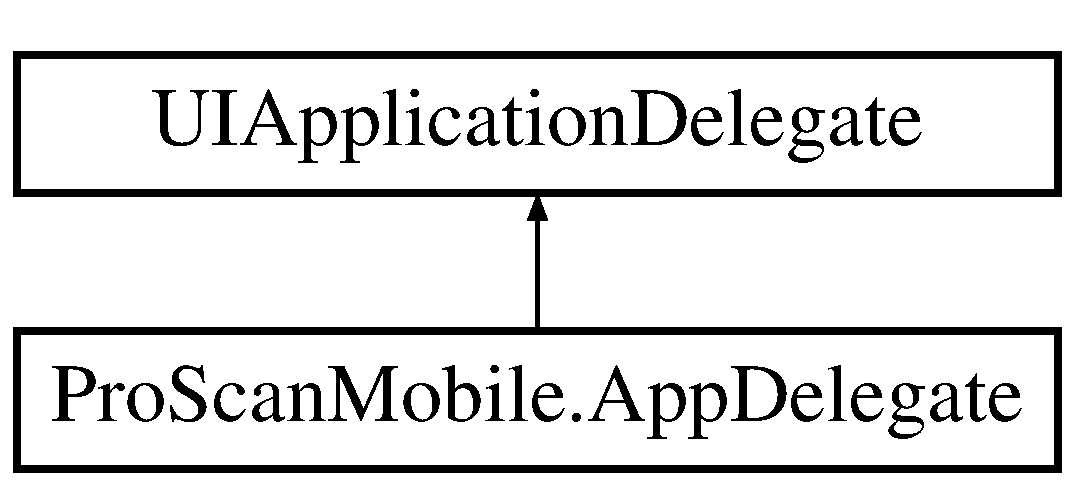
\includegraphics[height=2.000000cm]{class_pro_scan_mobile_1_1_app_delegate}
\end{center}
\end{figure}
\subsection*{Public Member Functions}
\begin{DoxyCompactItemize}
\item 
\hypertarget{class_pro_scan_mobile_1_1_app_delegate_a80c74e9bcf9109d07c26b0cd5bfd6894}{override bool {\bfseries Finished\-Launching} (U\-I\-Application app, N\-S\-Dictionary options)}\label{class_pro_scan_mobile_1_1_app_delegate_a80c74e9bcf9109d07c26b0cd5bfd6894}

\item 
\hypertarget{class_pro_scan_mobile_1_1_app_delegate_a9c4019ccd70667045aa01aed3ba052eb}{override void {\bfseries Perform\-Fetch} (U\-I\-Application application, Action$<$ U\-I\-Background\-Fetch\-Result $>$ completion\-Handler)}\label{class_pro_scan_mobile_1_1_app_delegate_a9c4019ccd70667045aa01aed3ba052eb}

\end{DoxyCompactItemize}


\subsection{Detailed Description}


Definition at line 13 of file App\-Delegate.\-cs.



The documentation for this class was generated from the following file\-:\begin{DoxyCompactItemize}
\item 
/\-Users/\-Jeff/\-Projects/\-Pro\-Scan\-Mobile+/\-Pro\-Scan\-Mobile+/App\-Delegate.\-cs\end{DoxyCompactItemize}

\hypertarget{class_pro_scan_mobile_1_1_application}{\section{Pro\-Scan\-Mobile.\-Application Class Reference}
\label{class_pro_scan_mobile_1_1_application}\index{Pro\-Scan\-Mobile.\-Application@{Pro\-Scan\-Mobile.\-Application}}
}


\subsection{Detailed Description}


Definition at line 9 of file Main.\-cs.



The documentation for this class was generated from the following file\-:\begin{DoxyCompactItemize}
\item 
/\-Users/\-Jeff/\-Projects/\-Pro\-Scan\-Mobile+/\-Pro\-Scan\-Mobile+/Main.\-cs\end{DoxyCompactItemize}

\hypertarget{class_pro_scan_mobile_1_1_custom_rec_cell}{\section{Pro\-Scan\-Mobile.\-Custom\-Rec\-Cell Class Reference}
\label{class_pro_scan_mobile_1_1_custom_rec_cell}\index{Pro\-Scan\-Mobile.\-Custom\-Rec\-Cell@{Pro\-Scan\-Mobile.\-Custom\-Rec\-Cell}}
}
Inheritance diagram for Pro\-Scan\-Mobile.\-Custom\-Rec\-Cell\-:\begin{figure}[H]
\begin{center}
\leavevmode
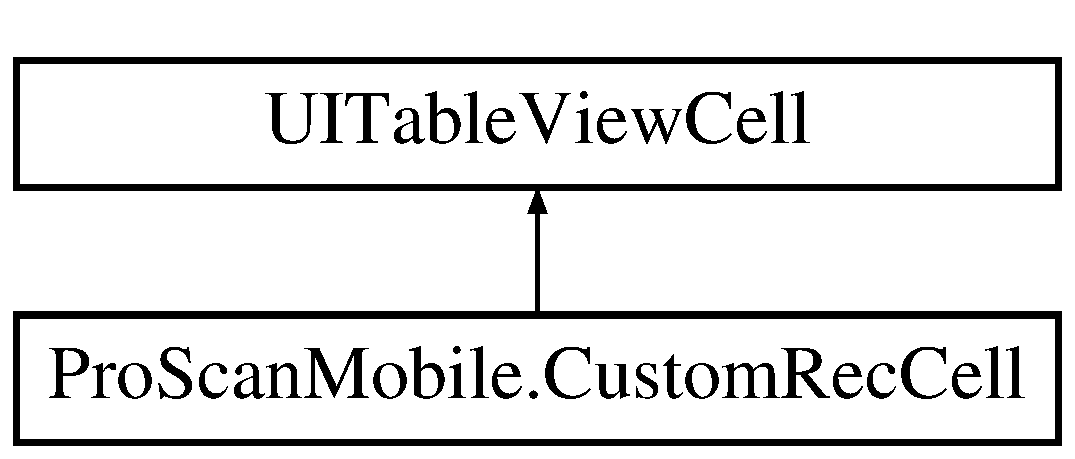
\includegraphics[height=2.000000cm]{class_pro_scan_mobile_1_1_custom_rec_cell}
\end{center}
\end{figure}
\subsection*{Public Member Functions}
\begin{DoxyCompactItemize}
\item 
\hypertarget{class_pro_scan_mobile_1_1_custom_rec_cell_a0d7e96ccd9839150b405e35e4f77ceee}{{\bfseries Custom\-Rec\-Cell} (N\-S\-String cell\-Id)}\label{class_pro_scan_mobile_1_1_custom_rec_cell_a0d7e96ccd9839150b405e35e4f77ceee}

\item 
\hypertarget{class_pro_scan_mobile_1_1_custom_rec_cell_a44e7381ca311c73532a3d3dfd284b357}{void {\bfseries Update\-Cell} (string file\-Name)}\label{class_pro_scan_mobile_1_1_custom_rec_cell_a44e7381ca311c73532a3d3dfd284b357}

\item 
\hypertarget{class_pro_scan_mobile_1_1_custom_rec_cell_abc36c0164227092e72a0698f2b2d4205}{override void {\bfseries Layout\-Subviews} ()}\label{class_pro_scan_mobile_1_1_custom_rec_cell_abc36c0164227092e72a0698f2b2d4205}

\item 
\hypertarget{class_pro_scan_mobile_1_1_custom_rec_cell_a1a3f6f587f1c1b5a15b64294252a90f2}{void {\bfseries Cell\-Changed} ()}\label{class_pro_scan_mobile_1_1_custom_rec_cell_a1a3f6f587f1c1b5a15b64294252a90f2}

\end{DoxyCompactItemize}
\subsection*{Properties}
\begin{DoxyCompactItemize}
\item 
\hypertarget{class_pro_scan_mobile_1_1_custom_rec_cell_a5584c336e04e83d965a9281b62192152}{A\-V\-Audio\-Player {\bfseries audio\-Player}\hspace{0.3cm}{\ttfamily  \mbox{[}get\mbox{]}}}\label{class_pro_scan_mobile_1_1_custom_rec_cell_a5584c336e04e83d965a9281b62192152}

\end{DoxyCompactItemize}


\subsection{Detailed Description}


Definition at line 10 of file Rec\-Table\-Cell.\-cs.



The documentation for this class was generated from the following file\-:\begin{DoxyCompactItemize}
\item 
/\-Users/\-Jeff/\-Projects/\-Pro\-Scan\-Mobile+/\-Pro\-Scan\-Mobile+/\-Classes/Rec\-Table\-Cell.\-cs\end{DoxyCompactItemize}

\hypertarget{class_pro_scan_mobile_1_1_custom_server_cell}{\section{Pro\-Scan\-Mobile.\-Custom\-Server\-Cell Class Reference}
\label{class_pro_scan_mobile_1_1_custom_server_cell}\index{Pro\-Scan\-Mobile.\-Custom\-Server\-Cell@{Pro\-Scan\-Mobile.\-Custom\-Server\-Cell}}
}
Inheritance diagram for Pro\-Scan\-Mobile.\-Custom\-Server\-Cell\-:\begin{figure}[H]
\begin{center}
\leavevmode
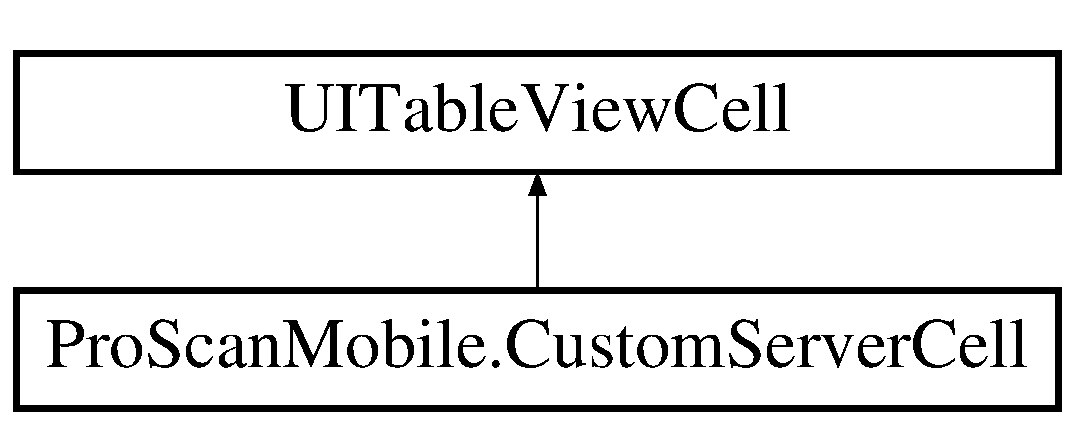
\includegraphics[height=2.000000cm]{class_pro_scan_mobile_1_1_custom_server_cell}
\end{center}
\end{figure}
\subsection*{Public Member Functions}
\begin{DoxyCompactItemize}
\item 
\hypertarget{class_pro_scan_mobile_1_1_custom_server_cell_ab16156002c5e173262fb48d26b3e0754}{{\bfseries Custom\-Server\-Cell} (N\-S\-String cell\-Id)}\label{class_pro_scan_mobile_1_1_custom_server_cell_ab16156002c5e173262fb48d26b3e0754}

\item 
\hypertarget{class_pro_scan_mobile_1_1_custom_server_cell_aa53cd659caf655d417602dddac91e28f}{void {\bfseries Update\-Cell} (U\-I\-Image image, string host, string port, string description, string country, string state, string county)}\label{class_pro_scan_mobile_1_1_custom_server_cell_aa53cd659caf655d417602dddac91e28f}

\item 
\hypertarget{class_pro_scan_mobile_1_1_custom_server_cell_a8dd06e9c800a56691ed2356d92e757c7}{override void {\bfseries Layout\-Subviews} ()}\label{class_pro_scan_mobile_1_1_custom_server_cell_a8dd06e9c800a56691ed2356d92e757c7}

\end{DoxyCompactItemize}


\subsection{Detailed Description}


Definition at line 8 of file Table\-Cell.\-cs.



The documentation for this class was generated from the following file\-:\begin{DoxyCompactItemize}
\item 
/\-Users/\-Jeff/\-Projects/\-Pro\-Scan\-Mobile+/\-Pro\-Scan\-Mobile+/\-Classes/Table\-Cell.\-cs\end{DoxyCompactItemize}

\hypertarget{class_pro_scan_mobile_1_1_encryption}{\section{Pro\-Scan\-Mobile.\-Encryption Class Reference}
\label{class_pro_scan_mobile_1_1_encryption}\index{Pro\-Scan\-Mobile.\-Encryption@{Pro\-Scan\-Mobile.\-Encryption}}
}
\subsection*{Public Member Functions}
\begin{DoxyCompactItemize}
\item 
\hypertarget{class_pro_scan_mobile_1_1_encryption_aa6fc2bbd504c6fad47e3198a909c40b2}{string {\bfseries Encrypt} (string p)}\label{class_pro_scan_mobile_1_1_encryption_aa6fc2bbd504c6fad47e3198a909c40b2}

\item 
\hypertarget{class_pro_scan_mobile_1_1_encryption_ab7d506d23f821c4ee65a2c10767f26b3}{string {\bfseries Decrypt} (string p)}\label{class_pro_scan_mobile_1_1_encryption_ab7d506d23f821c4ee65a2c10767f26b3}

\end{DoxyCompactItemize}


\subsection{Detailed Description}


Definition at line 7 of file Encryption.\-cs.



The documentation for this class was generated from the following file\-:\begin{DoxyCompactItemize}
\item 
/\-Users/\-Jeff/\-Projects/\-Pro\-Scan\-Mobile+/\-Pro\-Scan\-Mobile+/\-Classes/Encryption.\-cs\end{DoxyCompactItemize}

\hypertarget{class_pro_scan_mobile_1_1_network_connection}{\section{Pro\-Scan\-Mobile.\-Network\-Connection Class Reference}
\label{class_pro_scan_mobile_1_1_network_connection}\index{Pro\-Scan\-Mobile.\-Network\-Connection@{Pro\-Scan\-Mobile.\-Network\-Connection}}
}
\subsection*{Classes}
\begin{DoxyCompactItemize}
\item 
class \hyperlink{class_pro_scan_mobile_1_1_network_connection_1_1_state_object}{State\-Object}
\end{DoxyCompactItemize}
\subsection*{Public Types}
\begin{DoxyCompactItemize}
\item 
enum {\bfseries Connection\-Status} \{ {\bfseries Disconnected}, 
{\bfseries Connected}, 
{\bfseries Error}
 \}
\item 
enum {\bfseries Send\-Status} \{ {\bfseries Ok}, 
{\bfseries Error}
 \}
\item 
enum {\bfseries Receive\-Status} \{ {\bfseries Ok}, 
{\bfseries Error}
 \}
\item 
enum {\bfseries Login\-Status} \{ {\bfseries Logged\-In}, 
{\bfseries Logged\-Out}, 
{\bfseries Error}
 \}
\end{DoxyCompactItemize}
\subsection*{Public Member Functions}
\begin{DoxyCompactItemize}
\item 
\hypertarget{class_pro_scan_mobile_1_1_network_connection_abc9d352d3dd0d22920a0642e92ea6c72}{{\bfseries Network\-Connection} (string host, int port)}\label{class_pro_scan_mobile_1_1_network_connection_abc9d352d3dd0d22920a0642e92ea6c72}

\item 
\hypertarget{class_pro_scan_mobile_1_1_network_connection_a222c9e1fbec771a78830df002cc51856}{void {\bfseries Login} (string m)}\label{class_pro_scan_mobile_1_1_network_connection_a222c9e1fbec771a78830df002cc51856}

\item 
\hypertarget{class_pro_scan_mobile_1_1_network_connection_ab3102cf9e24372b296b5ded2fc528304}{void {\bfseries Log\-Out} (string m)}\label{class_pro_scan_mobile_1_1_network_connection_ab3102cf9e24372b296b5ded2fc528304}

\item 
\hypertarget{class_pro_scan_mobile_1_1_network_connection_a270b305a2b92ebac087cd567eb5536af}{void {\bfseries Close} ()}\label{class_pro_scan_mobile_1_1_network_connection_a270b305a2b92ebac087cd567eb5536af}

\item 
\hypertarget{class_pro_scan_mobile_1_1_network_connection_a9e9909205cd8025e1453548986f90cdf}{void {\bfseries Send} (string m)}\label{class_pro_scan_mobile_1_1_network_connection_a9e9909205cd8025e1453548986f90cdf}

\end{DoxyCompactItemize}
\subsection*{Public Attributes}
\begin{DoxyCompactItemize}
\item 
\hypertarget{class_pro_scan_mobile_1_1_network_connection_ade1283bd3d2eb2dca203b687a53c3fb8}{string {\bfseries \-\_\-connection\-Status\-Message}}\label{class_pro_scan_mobile_1_1_network_connection_ade1283bd3d2eb2dca203b687a53c3fb8}

\item 
\hypertarget{class_pro_scan_mobile_1_1_network_connection_a9c2c85fe4b8d57fdc40bf810d271a251}{string {\bfseries \-\_\-send\-Status\-Message}}\label{class_pro_scan_mobile_1_1_network_connection_a9c2c85fe4b8d57fdc40bf810d271a251}

\item 
\hypertarget{class_pro_scan_mobile_1_1_network_connection_a4572cd01ad183c20081e6aad39550225}{string {\bfseries \-\_\-receive\-Http\-Status\-Message}}\label{class_pro_scan_mobile_1_1_network_connection_a4572cd01ad183c20081e6aad39550225}

\item 
\hypertarget{class_pro_scan_mobile_1_1_network_connection_ae6a2dee68cef3d7c53cd29346cc21cb3}{string {\bfseries \-\_\-receive\-Data\-Status\-Message}}\label{class_pro_scan_mobile_1_1_network_connection_ae6a2dee68cef3d7c53cd29346cc21cb3}

\item 
\hypertarget{class_pro_scan_mobile_1_1_network_connection_a76ef797df5380e657a6071389627533b}{string {\bfseries \-\_\-login\-Status\-Message}}\label{class_pro_scan_mobile_1_1_network_connection_a76ef797df5380e657a6071389627533b}

\item 
\hypertarget{class_pro_scan_mobile_1_1_network_connection_a80a3d8fe1b4e582c82298db9f59c0326}{Date\-Time {\bfseries \-\_\-start\-Time}}\label{class_pro_scan_mobile_1_1_network_connection_a80a3d8fe1b4e582c82298db9f59c0326}

\end{DoxyCompactItemize}
\subsection*{Properties}
\begin{DoxyCompactItemize}
\item 
\hypertarget{class_pro_scan_mobile_1_1_network_connection_aff30c8cec509697e8a5a7e8a089f64a2}{Connection\-Status {\bfseries connection\-Status}\hspace{0.3cm}{\ttfamily  \mbox{[}get\mbox{]}}}\label{class_pro_scan_mobile_1_1_network_connection_aff30c8cec509697e8a5a7e8a089f64a2}

\item 
\hypertarget{class_pro_scan_mobile_1_1_network_connection_a6de7ff17ee23a814805bded88977313e}{Send\-Status {\bfseries send\-Status}\hspace{0.3cm}{\ttfamily  \mbox{[}get\mbox{]}}}\label{class_pro_scan_mobile_1_1_network_connection_a6de7ff17ee23a814805bded88977313e}

\item 
\hypertarget{class_pro_scan_mobile_1_1_network_connection_aad318a378efb9b9169180cba1237f30e}{Send\-Status {\bfseries receive\-Http\-Status}\hspace{0.3cm}{\ttfamily  \mbox{[}get\mbox{]}}}\label{class_pro_scan_mobile_1_1_network_connection_aad318a378efb9b9169180cba1237f30e}

\item 
\hypertarget{class_pro_scan_mobile_1_1_network_connection_aa090717a68fb052f707fa37f848c494e}{Send\-Status {\bfseries receive\-Data\-Status}\hspace{0.3cm}{\ttfamily  \mbox{[}get\mbox{]}}}\label{class_pro_scan_mobile_1_1_network_connection_aa090717a68fb052f707fa37f848c494e}

\item 
\hypertarget{class_pro_scan_mobile_1_1_network_connection_a2281ad7f92ca889cf7dddff0807b122f}{Login\-Status {\bfseries login\-Status}\hspace{0.3cm}{\ttfamily  \mbox{[}get\mbox{]}}}\label{class_pro_scan_mobile_1_1_network_connection_a2281ad7f92ca889cf7dddff0807b122f}

\item 
\hypertarget{class_pro_scan_mobile_1_1_network_connection_abdd15e53e48a54386878cefb7951060c}{Manual\-Reset\-Event {\bfseries connect\-Done}\hspace{0.3cm}{\ttfamily  \mbox{[}get\mbox{]}}}\label{class_pro_scan_mobile_1_1_network_connection_abdd15e53e48a54386878cefb7951060c}

\item 
\hypertarget{class_pro_scan_mobile_1_1_network_connection_af35886fc3bfcc83da9ef3571d99fa91c}{Manual\-Reset\-Event {\bfseries close\-Done}\hspace{0.3cm}{\ttfamily  \mbox{[}get\mbox{]}}}\label{class_pro_scan_mobile_1_1_network_connection_af35886fc3bfcc83da9ef3571d99fa91c}

\item 
\hypertarget{class_pro_scan_mobile_1_1_network_connection_aef0cbb620096d9dadb94b6a28c3ab442}{Manual\-Reset\-Event {\bfseries send\-Done}\hspace{0.3cm}{\ttfamily  \mbox{[}get\mbox{]}}}\label{class_pro_scan_mobile_1_1_network_connection_aef0cbb620096d9dadb94b6a28c3ab442}

\item 
\hypertarget{class_pro_scan_mobile_1_1_network_connection_a8fa14c62a4f4ebc6103e69b90ab70c69}{Manual\-Reset\-Event {\bfseries login\-Done}\hspace{0.3cm}{\ttfamily  \mbox{[}get\mbox{]}}}\label{class_pro_scan_mobile_1_1_network_connection_a8fa14c62a4f4ebc6103e69b90ab70c69}

\item 
\hypertarget{class_pro_scan_mobile_1_1_network_connection_acc628750f6cd703fca049defa5c64efa}{Manual\-Reset\-Event {\bfseries logout\-Done}\hspace{0.3cm}{\ttfamily  \mbox{[}get\mbox{]}}}\label{class_pro_scan_mobile_1_1_network_connection_acc628750f6cd703fca049defa5c64efa}

\item 
\hypertarget{class_pro_scan_mobile_1_1_network_connection_a30cce36c9657e0c5baa474ed4bb22ada}{int {\bfseries bytes\-Received}\hspace{0.3cm}{\ttfamily  \mbox{[}get\mbox{]}}}\label{class_pro_scan_mobile_1_1_network_connection_a30cce36c9657e0c5baa474ed4bb22ada}

\item 
\hypertarget{class_pro_scan_mobile_1_1_network_connection_a9c33fc95940f4a241c88e39e37882be1}{\hyperlink{class_pro_scan_mobile_1_1_read_write_buffer}{Read\-Write\-Buffer} {\bfseries connection\-Buffer}\hspace{0.3cm}{\ttfamily  \mbox{[}get\mbox{]}}}\label{class_pro_scan_mobile_1_1_network_connection_a9c33fc95940f4a241c88e39e37882be1}

\end{DoxyCompactItemize}


\subsection{Detailed Description}


Definition at line 13 of file Network\-Connection.\-cs.



The documentation for this class was generated from the following file\-:\begin{DoxyCompactItemize}
\item 
/\-Users/\-Jeff/\-Projects/\-Pro\-Scan\-Mobile+/\-Pro\-Scan\-Mobile+/\-Classes/Network\-Connection.\-cs\end{DoxyCompactItemize}

\hypertarget{class_pro_scan_mobile_1_1_read_write_buffer}{\section{Pro\-Scan\-Mobile.\-Read\-Write\-Buffer Class Reference}
\label{class_pro_scan_mobile_1_1_read_write_buffer}\index{Pro\-Scan\-Mobile.\-Read\-Write\-Buffer@{Pro\-Scan\-Mobile.\-Read\-Write\-Buffer}}
}
\subsection*{Public Member Functions}
\begin{DoxyCompactItemize}
\item 
\hypertarget{class_pro_scan_mobile_1_1_read_write_buffer_ae2f67e53253dd85cce783a53c0a08dc4}{{\bfseries Read\-Write\-Buffer} (int capacity)}\label{class_pro_scan_mobile_1_1_read_write_buffer_ae2f67e53253dd85cce783a53c0a08dc4}

\item 
\hypertarget{class_pro_scan_mobile_1_1_read_write_buffer_a8103075b1e58a61acbaa5392bd0d5e5f}{void {\bfseries Write} (byte\mbox{[}$\,$\mbox{]} data)}\label{class_pro_scan_mobile_1_1_read_write_buffer_a8103075b1e58a61acbaa5392bd0d5e5f}

\item 
\hypertarget{class_pro_scan_mobile_1_1_read_write_buffer_a1220f96aede4304e1815b03e55855f77}{byte\mbox{[}$\,$\mbox{]} {\bfseries Read} (int len, bool keep\-Data=false)}\label{class_pro_scan_mobile_1_1_read_write_buffer_a1220f96aede4304e1815b03e55855f77}

\end{DoxyCompactItemize}
\subsection*{Properties}
\begin{DoxyCompactItemize}
\item 
\hypertarget{class_pro_scan_mobile_1_1_read_write_buffer_a965102f5fcdaeb58b91f495a98a4cac1}{int {\bfseries Count}\hspace{0.3cm}{\ttfamily  \mbox{[}get\mbox{]}}}\label{class_pro_scan_mobile_1_1_read_write_buffer_a965102f5fcdaeb58b91f495a98a4cac1}

\item 
\hypertarget{class_pro_scan_mobile_1_1_read_write_buffer_a9d6ab0f4c9bdbf0c43e7257ca598795d}{byte {\bfseries this\mbox{[}int index\mbox{]}}\hspace{0.3cm}{\ttfamily  \mbox{[}get\mbox{]}}}\label{class_pro_scan_mobile_1_1_read_write_buffer_a9d6ab0f4c9bdbf0c43e7257ca598795d}

\item 
\hypertarget{class_pro_scan_mobile_1_1_read_write_buffer_a615a176a8c5115ee8add73f7116b0a30}{I\-Enumerable {\bfseries Bytes}\hspace{0.3cm}{\ttfamily  \mbox{[}get\mbox{]}}}\label{class_pro_scan_mobile_1_1_read_write_buffer_a615a176a8c5115ee8add73f7116b0a30}

\end{DoxyCompactItemize}


\subsection{Detailed Description}


Definition at line 6 of file Read\-Write\-Buffer.\-cs.



The documentation for this class was generated from the following file\-:\begin{DoxyCompactItemize}
\item 
/\-Users/\-Jeff/\-Projects/\-Pro\-Scan\-Mobile+/\-Pro\-Scan\-Mobile+/\-Classes/Read\-Write\-Buffer.\-cs\end{DoxyCompactItemize}

\hypertarget{class_pro_scan_mobile_1_1_rec_table_item}{\section{Pro\-Scan\-Mobile.\-Rec\-Table\-Item Class Reference}
\label{class_pro_scan_mobile_1_1_rec_table_item}\index{Pro\-Scan\-Mobile.\-Rec\-Table\-Item@{Pro\-Scan\-Mobile.\-Rec\-Table\-Item}}
}
\subsection*{Public Member Functions}
\begin{DoxyCompactItemize}
\item 
\hypertarget{class_pro_scan_mobile_1_1_rec_table_item_af836481c2bc1b8a31c6f445a2e9f2fc4}{{\bfseries Rec\-Table\-Item} (string heading)}\label{class_pro_scan_mobile_1_1_rec_table_item_af836481c2bc1b8a31c6f445a2e9f2fc4}

\end{DoxyCompactItemize}
\subsection*{Protected Attributes}
\begin{DoxyCompactItemize}
\item 
\hypertarget{class_pro_scan_mobile_1_1_rec_table_item_a93f4d1d5f688e7b6d8b6a7a8e015e9df}{U\-I\-Table\-View\-Cell\-Style {\bfseries cell\-Style} = U\-I\-Table\-View\-Cell\-Style.\-Default}\label{class_pro_scan_mobile_1_1_rec_table_item_a93f4d1d5f688e7b6d8b6a7a8e015e9df}

\item 
\hypertarget{class_pro_scan_mobile_1_1_rec_table_item_ab59f5fb9e815c173550ae6bfc8691f11}{U\-I\-Table\-View\-Cell\-Accessory {\bfseries cell\-Accessory} = U\-I\-Table\-View\-Cell\-Accessory.\-None}\label{class_pro_scan_mobile_1_1_rec_table_item_ab59f5fb9e815c173550ae6bfc8691f11}

\end{DoxyCompactItemize}
\subsection*{Properties}
\begin{DoxyCompactItemize}
\item 
\hypertarget{class_pro_scan_mobile_1_1_rec_table_item_a986fbc59f5cd9776d3ad721a6319bdf9}{string {\bfseries File}\hspace{0.3cm}{\ttfamily  \mbox{[}get, set\mbox{]}}}\label{class_pro_scan_mobile_1_1_rec_table_item_a986fbc59f5cd9776d3ad721a6319bdf9}

\item 
\hypertarget{class_pro_scan_mobile_1_1_rec_table_item_a09050c401c18bc892188a256fda21591}{U\-I\-Table\-View\-Cell\-Style {\bfseries Cell\-Style}\hspace{0.3cm}{\ttfamily  \mbox{[}get, set\mbox{]}}}\label{class_pro_scan_mobile_1_1_rec_table_item_a09050c401c18bc892188a256fda21591}

\item 
\hypertarget{class_pro_scan_mobile_1_1_rec_table_item_a908bcc04b2442097c0f56535fe259702}{U\-I\-Table\-View\-Cell\-Accessory {\bfseries Cell\-Accessory}\hspace{0.3cm}{\ttfamily  \mbox{[}get, set\mbox{]}}}\label{class_pro_scan_mobile_1_1_rec_table_item_a908bcc04b2442097c0f56535fe259702}

\end{DoxyCompactItemize}


\subsection{Detailed Description}


Definition at line 6 of file Rec\-Table\-Item.\-cs.



The documentation for this class was generated from the following file\-:\begin{DoxyCompactItemize}
\item 
/\-Users/\-Jeff/\-Projects/\-Pro\-Scan\-Mobile+/\-Pro\-Scan\-Mobile+/\-Classes/Rec\-Table\-Item.\-cs\end{DoxyCompactItemize}

\hypertarget{class_pro_scan_mobile_1_1_rec_table_source}{\section{Pro\-Scan\-Mobile.\-Rec\-Table\-Source Class Reference}
\label{class_pro_scan_mobile_1_1_rec_table_source}\index{Pro\-Scan\-Mobile.\-Rec\-Table\-Source@{Pro\-Scan\-Mobile.\-Rec\-Table\-Source}}
}
Inheritance diagram for Pro\-Scan\-Mobile.\-Rec\-Table\-Source\-:\begin{figure}[H]
\begin{center}
\leavevmode
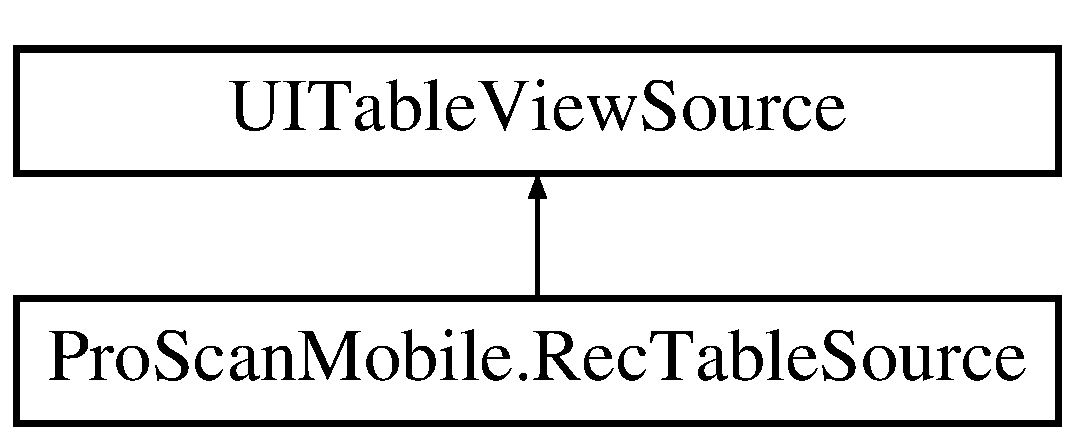
\includegraphics[height=2.000000cm]{class_pro_scan_mobile_1_1_rec_table_source}
\end{center}
\end{figure}
\subsection*{Public Member Functions}
\begin{DoxyCompactItemize}
\item 
\hypertarget{class_pro_scan_mobile_1_1_rec_table_source_ab73f5cf14799e5ef7eae84df12566671}{{\bfseries Rec\-Table\-Source} (string\mbox{[}$\,$\mbox{]} items)}\label{class_pro_scan_mobile_1_1_rec_table_source_ab73f5cf14799e5ef7eae84df12566671}

\item 
\hypertarget{class_pro_scan_mobile_1_1_rec_table_source_ad731ea1b0e706282e863c273dbbc4316}{override float {\bfseries Get\-Height\-For\-Row} (U\-I\-Table\-View table\-View, N\-S\-Index\-Path index\-Path)}\label{class_pro_scan_mobile_1_1_rec_table_source_ad731ea1b0e706282e863c273dbbc4316}

\item 
\hypertarget{class_pro_scan_mobile_1_1_rec_table_source_a0472474af7c7cbaa6bb34f72d9548067}{override string {\bfseries Title\-For\-Header} (U\-I\-Table\-View table\-View, int section)}\label{class_pro_scan_mobile_1_1_rec_table_source_a0472474af7c7cbaa6bb34f72d9548067}

\item 
\hypertarget{class_pro_scan_mobile_1_1_rec_table_source_abb9ecbeca34ad656249585527a19289b}{override U\-I\-Table\-View\-Cell {\bfseries Get\-Cell} (U\-I\-Table\-View table\-View, Mono\-Touch.\-Foundation.\-N\-S\-Index\-Path index\-Path)}\label{class_pro_scan_mobile_1_1_rec_table_source_abb9ecbeca34ad656249585527a19289b}

\item 
\hypertarget{class_pro_scan_mobile_1_1_rec_table_source_a72b2c22fe65636fcdd76a6b00806bc31}{override void {\bfseries Row\-Selected} (U\-I\-Table\-View table\-View, N\-S\-Index\-Path index\-Path)}\label{class_pro_scan_mobile_1_1_rec_table_source_a72b2c22fe65636fcdd76a6b00806bc31}

\item 
\hypertarget{class_pro_scan_mobile_1_1_rec_table_source_aae1433be7b808d9b57768197f8f2b999}{override void {\bfseries Commit\-Editing\-Style} (U\-I\-Table\-View table\-View, U\-I\-Table\-View\-Cell\-Editing\-Style editing\-Style, Mono\-Touch.\-Foundation.\-N\-S\-Index\-Path index\-Path)}\label{class_pro_scan_mobile_1_1_rec_table_source_aae1433be7b808d9b57768197f8f2b999}

\item 
\hypertarget{class_pro_scan_mobile_1_1_rec_table_source_ad0a7ec7a1c8d190996204d21f5e042a1}{override int {\bfseries Rows\-In\-Section} (U\-I\-Table\-View tableview, int section)}\label{class_pro_scan_mobile_1_1_rec_table_source_ad0a7ec7a1c8d190996204d21f5e042a1}

\item 
\hypertarget{class_pro_scan_mobile_1_1_rec_table_source_a6878d721d17d3cc38f872308988dec7f}{override bool {\bfseries Can\-Edit\-Row} (U\-I\-Table\-View table\-View, N\-S\-Index\-Path index\-Path)}\label{class_pro_scan_mobile_1_1_rec_table_source_a6878d721d17d3cc38f872308988dec7f}

\item 
\hypertarget{class_pro_scan_mobile_1_1_rec_table_source_aab670ca701c9e2c1a9c0f352b1606dc2}{override string {\bfseries Title\-For\-Delete\-Confirmation} (U\-I\-Table\-View table\-View, N\-S\-Index\-Path index\-Path)}\label{class_pro_scan_mobile_1_1_rec_table_source_aab670ca701c9e2c1a9c0f352b1606dc2}

\end{DoxyCompactItemize}


\subsection{Detailed Description}


Definition at line 11 of file Rec\-Table\-Source.\-cs.



The documentation for this class was generated from the following file\-:\begin{DoxyCompactItemize}
\item 
/\-Users/\-Jeff/\-Projects/\-Pro\-Scan\-Mobile+/\-Pro\-Scan\-Mobile+/\-Classes/Rec\-Table\-Source.\-cs\end{DoxyCompactItemize}

\hypertarget{class_pro_scan_mobile_1_1_scanner_audio}{\section{Pro\-Scan\-Mobile.\-Scanner\-Audio Class Reference}
\label{class_pro_scan_mobile_1_1_scanner_audio}\index{Pro\-Scan\-Mobile.\-Scanner\-Audio@{Pro\-Scan\-Mobile.\-Scanner\-Audio}}
}
\subsection*{Public Member Functions}
\begin{DoxyCompactItemize}
\item 
\hypertarget{class_pro_scan_mobile_1_1_scanner_audio_a0bf4a22616d20987c42335737acba9ba}{void {\bfseries Dispose} ()}\label{class_pro_scan_mobile_1_1_scanner_audio_a0bf4a22616d20987c42335737acba9ba}

\item 
\hypertarget{class_pro_scan_mobile_1_1_scanner_audio_a14667ddc0ec45ddf2d0b8f1e75401d61}{void {\bfseries Prepare\-Output\-To\-File} ()}\label{class_pro_scan_mobile_1_1_scanner_audio_a14667ddc0ec45ddf2d0b8f1e75401d61}

\item 
\hypertarget{class_pro_scan_mobile_1_1_scanner_audio_a68f3c557cb4f1a304037a59b14190c3a}{void {\bfseries Stop\-Output\-To\-File} ()}\label{class_pro_scan_mobile_1_1_scanner_audio_a68f3c557cb4f1a304037a59b14190c3a}

\item 
\hypertarget{class_pro_scan_mobile_1_1_scanner_audio_af5f0f970d508baf9bd732bcbd74fe1a1}{void {\bfseries process\-Data} (byte\mbox{[}$\,$\mbox{]} message, int message\-Length)}\label{class_pro_scan_mobile_1_1_scanner_audio_af5f0f970d508baf9bd732bcbd74fe1a1}

\end{DoxyCompactItemize}
\subsection*{Properties}
\begin{DoxyCompactItemize}
\item 
\hypertarget{class_pro_scan_mobile_1_1_scanner_audio_af9084593f78d2df56b8e5053c9588146}{string {\bfseries scanner\-Audio\-\_\-\-Mpeg}\hspace{0.3cm}{\ttfamily  \mbox{[}get\mbox{]}}}\label{class_pro_scan_mobile_1_1_scanner_audio_af9084593f78d2df56b8e5053c9588146}

\item 
\hypertarget{class_pro_scan_mobile_1_1_scanner_audio_a082206408783224924ce41f41bbaa0b1}{string {\bfseries scanner\-Audio\-\_\-\-Freq}\hspace{0.3cm}{\ttfamily  \mbox{[}get\mbox{]}}}\label{class_pro_scan_mobile_1_1_scanner_audio_a082206408783224924ce41f41bbaa0b1}

\item 
\hypertarget{class_pro_scan_mobile_1_1_scanner_audio_a3f4c416df6ce416ee528980324f72929}{string {\bfseries scanner\-Audio\-\_\-\-Rate}\hspace{0.3cm}{\ttfamily  \mbox{[}get\mbox{]}}}\label{class_pro_scan_mobile_1_1_scanner_audio_a3f4c416df6ce416ee528980324f72929}

\item 
\hypertarget{class_pro_scan_mobile_1_1_scanner_audio_a0cdaf7cbb44b2b7270cdcc2a7024ba47}{bool {\bfseries scanner\-Audio\-\_\-\-Buffering}\hspace{0.3cm}{\ttfamily  \mbox{[}get\mbox{]}}}\label{class_pro_scan_mobile_1_1_scanner_audio_a0cdaf7cbb44b2b7270cdcc2a7024ba47}

\end{DoxyCompactItemize}


\subsection{Detailed Description}


Definition at line 8 of file Scanner\-Audio.\-cs.



The documentation for this class was generated from the following file\-:\begin{DoxyCompactItemize}
\item 
/\-Users/\-Jeff/\-Projects/\-Pro\-Scan\-Mobile+/\-Pro\-Scan\-Mobile+/\-Classes/Scanner\-Audio.\-cs\end{DoxyCompactItemize}

\hypertarget{class_pro_scan_mobile_1_1_scanner_screen}{\section{Pro\-Scan\-Mobile.\-Scanner\-Screen Class Reference}
\label{class_pro_scan_mobile_1_1_scanner_screen}\index{Pro\-Scan\-Mobile.\-Scanner\-Screen@{Pro\-Scan\-Mobile.\-Scanner\-Screen}}
}
\subsection*{Public Member Functions}
\begin{DoxyCompactItemize}
\item 
\hypertarget{class_pro_scan_mobile_1_1_scanner_screen_af9589000b217a6fb2406ceab88007866}{void {\bfseries Dispose} ()}\label{class_pro_scan_mobile_1_1_scanner_screen_af9589000b217a6fb2406ceab88007866}

\item 
\hypertarget{class_pro_scan_mobile_1_1_scanner_screen_a56aa170a775179044764775cdc467e22}{void {\bfseries process\-Data} (byte\mbox{[}$\,$\mbox{]} message, int message\-Length)}\label{class_pro_scan_mobile_1_1_scanner_screen_a56aa170a775179044764775cdc467e22}

\end{DoxyCompactItemize}
\subsection*{Properties}
\begin{DoxyCompactItemize}
\item 
\hypertarget{class_pro_scan_mobile_1_1_scanner_screen_a312e1d743253507427858c4b05c9a2d7}{string {\bfseries scanner\-Screen\-\_\-\-Model}\hspace{0.3cm}{\ttfamily  \mbox{[}get\mbox{]}}}\label{class_pro_scan_mobile_1_1_scanner_screen_a312e1d743253507427858c4b05c9a2d7}

\item 
\hypertarget{class_pro_scan_mobile_1_1_scanner_screen_aa2ed3517186b388525c0c66c172ec78a}{int {\bfseries scanner\-Screen\-\_\-\-Signal}\hspace{0.3cm}{\ttfamily  \mbox{[}get\mbox{]}}}\label{class_pro_scan_mobile_1_1_scanner_screen_aa2ed3517186b388525c0c66c172ec78a}

\item 
\hypertarget{class_pro_scan_mobile_1_1_scanner_screen_a973422ca8f9475dfee5a0dd54d010fd6}{string {\bfseries scanner\-Screen\-\_\-\-Line1}\hspace{0.3cm}{\ttfamily  \mbox{[}get\mbox{]}}}\label{class_pro_scan_mobile_1_1_scanner_screen_a973422ca8f9475dfee5a0dd54d010fd6}

\item 
\hypertarget{class_pro_scan_mobile_1_1_scanner_screen_a7c3dc8baf7564a16b9139b4929a242ea}{string {\bfseries scanner\-Screen\-\_\-\-Line2}\hspace{0.3cm}{\ttfamily  \mbox{[}get\mbox{]}}}\label{class_pro_scan_mobile_1_1_scanner_screen_a7c3dc8baf7564a16b9139b4929a242ea}

\item 
\hypertarget{class_pro_scan_mobile_1_1_scanner_screen_a68eb503120ff2fa45eab0784af303880}{string {\bfseries scanner\-Screen\-\_\-\-Line3}\hspace{0.3cm}{\ttfamily  \mbox{[}get\mbox{]}}}\label{class_pro_scan_mobile_1_1_scanner_screen_a68eb503120ff2fa45eab0784af303880}

\item 
\hypertarget{class_pro_scan_mobile_1_1_scanner_screen_a5b6da547ee1c350dd7c8129af2af9319}{string {\bfseries scanner\-Screen\-\_\-\-Line4}\hspace{0.3cm}{\ttfamily  \mbox{[}get\mbox{]}}}\label{class_pro_scan_mobile_1_1_scanner_screen_a5b6da547ee1c350dd7c8129af2af9319}

\item 
\hypertarget{class_pro_scan_mobile_1_1_scanner_screen_a13994fe064768843a55197cf08b30f2d}{string {\bfseries scanner\-Screen\-\_\-\-Line5}\hspace{0.3cm}{\ttfamily  \mbox{[}get\mbox{]}}}\label{class_pro_scan_mobile_1_1_scanner_screen_a13994fe064768843a55197cf08b30f2d}

\end{DoxyCompactItemize}


\subsection{Detailed Description}


Definition at line 7 of file Scanner\-Screen.\-cs.



The documentation for this class was generated from the following file\-:\begin{DoxyCompactItemize}
\item 
/\-Users/\-Jeff/\-Projects/\-Pro\-Scan\-Mobile+/\-Pro\-Scan\-Mobile+/\-Classes/Scanner\-Screen.\-cs\end{DoxyCompactItemize}

\hypertarget{class_pro_scan_mobile_1_1vc_options_screen_1_1_server_details}{\section{Pro\-Scan\-Mobile.\-vc\-Options\-Screen.\-Server\-Details Class Reference}
\label{class_pro_scan_mobile_1_1vc_options_screen_1_1_server_details}\index{Pro\-Scan\-Mobile.\-vc\-Options\-Screen.\-Server\-Details@{Pro\-Scan\-Mobile.\-vc\-Options\-Screen.\-Server\-Details}}
}
\subsection*{Properties}
\begin{DoxyCompactItemize}
\item 
\hypertarget{class_pro_scan_mobile_1_1vc_options_screen_1_1_server_details_ae2b39ca21c9050a6a96bb15c7ddfdf79}{string {\bfseries open}\hspace{0.3cm}{\ttfamily  \mbox{[}get, set\mbox{]}}}\label{class_pro_scan_mobile_1_1vc_options_screen_1_1_server_details_ae2b39ca21c9050a6a96bb15c7ddfdf79}

\item 
\hypertarget{class_pro_scan_mobile_1_1vc_options_screen_1_1_server_details_a762d9eae22a69429c6881f8b7710fb67}{string {\bfseries host}\hspace{0.3cm}{\ttfamily  \mbox{[}get, set\mbox{]}}}\label{class_pro_scan_mobile_1_1vc_options_screen_1_1_server_details_a762d9eae22a69429c6881f8b7710fb67}

\item 
\hypertarget{class_pro_scan_mobile_1_1vc_options_screen_1_1_server_details_a657f20b977f68b9a6324f1da080b5ef9}{string {\bfseries port}\hspace{0.3cm}{\ttfamily  \mbox{[}get, set\mbox{]}}}\label{class_pro_scan_mobile_1_1vc_options_screen_1_1_server_details_a657f20b977f68b9a6324f1da080b5ef9}

\item 
\hypertarget{class_pro_scan_mobile_1_1vc_options_screen_1_1_server_details_a384687ca8c0040814629776ea291f6fc}{string {\bfseries desc}\hspace{0.3cm}{\ttfamily  \mbox{[}get, set\mbox{]}}}\label{class_pro_scan_mobile_1_1vc_options_screen_1_1_server_details_a384687ca8c0040814629776ea291f6fc}

\item 
\hypertarget{class_pro_scan_mobile_1_1vc_options_screen_1_1_server_details_aa916419a83933de397736bdfc12a9fb6}{string {\bfseries country}\hspace{0.3cm}{\ttfamily  \mbox{[}get, set\mbox{]}}}\label{class_pro_scan_mobile_1_1vc_options_screen_1_1_server_details_aa916419a83933de397736bdfc12a9fb6}

\item 
\hypertarget{class_pro_scan_mobile_1_1vc_options_screen_1_1_server_details_a651086eb83f2e749f8dc415436a55d40}{string {\bfseries state}\hspace{0.3cm}{\ttfamily  \mbox{[}get, set\mbox{]}}}\label{class_pro_scan_mobile_1_1vc_options_screen_1_1_server_details_a651086eb83f2e749f8dc415436a55d40}

\item 
\hypertarget{class_pro_scan_mobile_1_1vc_options_screen_1_1_server_details_aa92f63735ffeee1b3aaaa7fd04cd0c67}{string {\bfseries county}\hspace{0.3cm}{\ttfamily  \mbox{[}get, set\mbox{]}}}\label{class_pro_scan_mobile_1_1vc_options_screen_1_1_server_details_aa92f63735ffeee1b3aaaa7fd04cd0c67}

\end{DoxyCompactItemize}


\subsection{Detailed Description}


Definition at line 56 of file vc\-Options\-Screen.\-cs.



The documentation for this class was generated from the following file\-:\begin{DoxyCompactItemize}
\item 
/\-Users/\-Jeff/\-Projects/\-Pro\-Scan\-Mobile+/\-Pro\-Scan\-Mobile+/\-Screens/vc\-Options\-Screen.\-cs\end{DoxyCompactItemize}

\hypertarget{class_pro_scan_mobile_1_1vc_options_screen_1_1_servers}{\section{Pro\-Scan\-Mobile.\-vc\-Options\-Screen.\-Servers Class Reference}
\label{class_pro_scan_mobile_1_1vc_options_screen_1_1_servers}\index{Pro\-Scan\-Mobile.\-vc\-Options\-Screen.\-Servers@{Pro\-Scan\-Mobile.\-vc\-Options\-Screen.\-Servers}}
}
\subsection*{Properties}
\begin{DoxyCompactItemize}
\item 
\hypertarget{class_pro_scan_mobile_1_1vc_options_screen_1_1_servers_ab91832dd19b800740986a06b64affe16}{List$<$ \hyperlink{class_pro_scan_mobile_1_1vc_options_screen_1_1_server_details}{Server\-Details} $>$ {\bfseries Server\-List}\hspace{0.3cm}{\ttfamily  \mbox{[}get, set\mbox{]}}}\label{class_pro_scan_mobile_1_1vc_options_screen_1_1_servers_ab91832dd19b800740986a06b64affe16}

\end{DoxyCompactItemize}


\subsection{Detailed Description}


Definition at line 49 of file vc\-Options\-Screen.\-cs.



The documentation for this class was generated from the following file\-:\begin{DoxyCompactItemize}
\item 
/\-Users/\-Jeff/\-Projects/\-Pro\-Scan\-Mobile+/\-Pro\-Scan\-Mobile+/\-Screens/vc\-Options\-Screen.\-cs\end{DoxyCompactItemize}

\hypertarget{class_pro_scan_mobile_1_1vc_options_screen_1_1_settings}{\section{Pro\-Scan\-Mobile.\-vc\-Options\-Screen.\-Settings Class Reference}
\label{class_pro_scan_mobile_1_1vc_options_screen_1_1_settings}\index{Pro\-Scan\-Mobile.\-vc\-Options\-Screen.\-Settings@{Pro\-Scan\-Mobile.\-vc\-Options\-Screen.\-Settings}}
}
\subsection*{Properties}
\begin{DoxyCompactItemize}
\item 
\hypertarget{class_pro_scan_mobile_1_1vc_options_screen_1_1_settings_aaeed636d7ea28816cd217c619760a78f}{List$<$ \hyperlink{class_pro_scan_mobile_1_1vc_options_screen_1_1_settings_details}{Settings\-Details} $>$ {\bfseries Settings\-List}\hspace{0.3cm}{\ttfamily  \mbox{[}get, set\mbox{]}}}\label{class_pro_scan_mobile_1_1vc_options_screen_1_1_settings_aaeed636d7ea28816cd217c619760a78f}

\end{DoxyCompactItemize}


\subsection{Detailed Description}


Definition at line 32 of file vc\-Options\-Screen.\-cs.



The documentation for this class was generated from the following file\-:\begin{DoxyCompactItemize}
\item 
/\-Users/\-Jeff/\-Projects/\-Pro\-Scan\-Mobile+/\-Pro\-Scan\-Mobile+/\-Screens/vc\-Options\-Screen.\-cs\end{DoxyCompactItemize}

\hypertarget{class_pro_scan_mobile_1_1vc_options_screen_1_1_settings_details}{\section{Pro\-Scan\-Mobile.\-vc\-Options\-Screen.\-Settings\-Details Class Reference}
\label{class_pro_scan_mobile_1_1vc_options_screen_1_1_settings_details}\index{Pro\-Scan\-Mobile.\-vc\-Options\-Screen.\-Settings\-Details@{Pro\-Scan\-Mobile.\-vc\-Options\-Screen.\-Settings\-Details}}
}
\subsection*{Properties}
\begin{DoxyCompactItemize}
\item 
\hypertarget{class_pro_scan_mobile_1_1vc_options_screen_1_1_settings_details_ad279dd73ba9c5d76369deee0aedd3c77}{string {\bfseries host}\hspace{0.3cm}{\ttfamily  \mbox{[}get, set\mbox{]}}}\label{class_pro_scan_mobile_1_1vc_options_screen_1_1_settings_details_ad279dd73ba9c5d76369deee0aedd3c77}

\item 
\hypertarget{class_pro_scan_mobile_1_1vc_options_screen_1_1_settings_details_a15165280af6125718979d0dd55e89798}{int {\bfseries port}\hspace{0.3cm}{\ttfamily  \mbox{[}get, set\mbox{]}}}\label{class_pro_scan_mobile_1_1vc_options_screen_1_1_settings_details_a15165280af6125718979d0dd55e89798}

\item 
\hypertarget{class_pro_scan_mobile_1_1vc_options_screen_1_1_settings_details_ac53111112550aebca182a06f9f966e40}{bool {\bfseries auto}\hspace{0.3cm}{\ttfamily  \mbox{[}get, set\mbox{]}}}\label{class_pro_scan_mobile_1_1vc_options_screen_1_1_settings_details_ac53111112550aebca182a06f9f966e40}

\item 
\hypertarget{class_pro_scan_mobile_1_1vc_options_screen_1_1_settings_details_a15c097ac65b52dce1974eecb0cdc4c3c}{string {\bfseries pass}\hspace{0.3cm}{\ttfamily  \mbox{[}get, set\mbox{]}}}\label{class_pro_scan_mobile_1_1vc_options_screen_1_1_settings_details_a15c097ac65b52dce1974eecb0cdc4c3c}

\end{DoxyCompactItemize}


\subsection{Detailed Description}


Definition at line 39 of file vc\-Options\-Screen.\-cs.



The documentation for this class was generated from the following file\-:\begin{DoxyCompactItemize}
\item 
/\-Users/\-Jeff/\-Projects/\-Pro\-Scan\-Mobile+/\-Pro\-Scan\-Mobile+/\-Screens/vc\-Options\-Screen.\-cs\end{DoxyCompactItemize}

\hypertarget{class_pro_scan_mobile_1_1_network_connection_1_1_state_object}{\section{Pro\-Scan\-Mobile.\-Network\-Connection.\-State\-Object Class Reference}
\label{class_pro_scan_mobile_1_1_network_connection_1_1_state_object}\index{Pro\-Scan\-Mobile.\-Network\-Connection.\-State\-Object@{Pro\-Scan\-Mobile.\-Network\-Connection.\-State\-Object}}
}
\subsection*{Public Attributes}
\begin{DoxyCompactItemize}
\item 
\hypertarget{class_pro_scan_mobile_1_1_network_connection_1_1_state_object_ad520e994b85670d04f24db5976720e3b}{Socket {\bfseries work\-Socket} = null}\label{class_pro_scan_mobile_1_1_network_connection_1_1_state_object_ad520e994b85670d04f24db5976720e3b}

\item 
\hypertarget{class_pro_scan_mobile_1_1_network_connection_1_1_state_object_a7dd7b0f84ec17a00ca03a0b53e9615c6}{const int {\bfseries Buffer\-Size} = 65535}\label{class_pro_scan_mobile_1_1_network_connection_1_1_state_object_a7dd7b0f84ec17a00ca03a0b53e9615c6}

\item 
\hypertarget{class_pro_scan_mobile_1_1_network_connection_1_1_state_object_aaa4a50080195b13f6a9a72edab38765d}{byte\mbox{[}$\,$\mbox{]} {\bfseries buffer} = new byte\mbox{[}Buffer\-Size\mbox{]}}\label{class_pro_scan_mobile_1_1_network_connection_1_1_state_object_aaa4a50080195b13f6a9a72edab38765d}

\end{DoxyCompactItemize}


\subsection{Detailed Description}


Definition at line 82 of file Network\-Connection.\-cs.



The documentation for this class was generated from the following file\-:\begin{DoxyCompactItemize}
\item 
/\-Users/\-Jeff/\-Projects/\-Pro\-Scan\-Mobile+/\-Pro\-Scan\-Mobile+/\-Classes/Network\-Connection.\-cs\end{DoxyCompactItemize}

\hypertarget{class_pro_scan_mobile_1_1_streaming_playback_v2}{\section{Pro\-Scan\-Mobile.\-Streaming\-Playback\-V2 Class Reference}
\label{class_pro_scan_mobile_1_1_streaming_playback_v2}\index{Pro\-Scan\-Mobile.\-Streaming\-Playback\-V2@{Pro\-Scan\-Mobile.\-Streaming\-Playback\-V2}}
}
\subsection*{Public Member Functions}
\begin{DoxyCompactItemize}
\item 
\hypertarget{class_pro_scan_mobile_1_1_streaming_playback_v2_a5e7cffcd39a6de557f29b791836f5ad3}{void {\bfseries Parse\-Bytes} (byte\mbox{[}$\,$\mbox{]} buffer, int count, bool discontinuity)}\label{class_pro_scan_mobile_1_1_streaming_playback_v2_a5e7cffcd39a6de557f29b791836f5ad3}

\item 
\hypertarget{class_pro_scan_mobile_1_1_streaming_playback_v2_a6e9291be5fcb6b99732cf032bd72db90}{void {\bfseries Dispose} ()}\label{class_pro_scan_mobile_1_1_streaming_playback_v2_a6e9291be5fcb6b99732cf032bd72db90}

\item 
\hypertarget{class_pro_scan_mobile_1_1_streaming_playback_v2_a73a502415b5f5458b383d7d74382b3d5}{void {\bfseries Start} ()}\label{class_pro_scan_mobile_1_1_streaming_playback_v2_a73a502415b5f5458b383d7d74382b3d5}

\end{DoxyCompactItemize}


\subsection{Detailed Description}


Definition at line 10 of file Streaming\-Playback\-V2.\-cs.



The documentation for this class was generated from the following file\-:\begin{DoxyCompactItemize}
\item 
/\-Users/\-Jeff/\-Projects/\-Pro\-Scan\-Mobile+/\-Pro\-Scan\-Mobile+/\-Classes/Streaming\-Playback\-V2.\-cs\end{DoxyCompactItemize}

\hypertarget{class_pro_scan_mobile_1_1_table_item}{\section{Pro\-Scan\-Mobile.\-Table\-Item Class Reference}
\label{class_pro_scan_mobile_1_1_table_item}\index{Pro\-Scan\-Mobile.\-Table\-Item@{Pro\-Scan\-Mobile.\-Table\-Item}}
}
\subsection*{Public Member Functions}
\begin{DoxyCompactItemize}
\item 
\hypertarget{class_pro_scan_mobile_1_1_table_item_a7cb46224e5cfb1be1b562a8e23de752e}{{\bfseries Table\-Item} (string heading)}\label{class_pro_scan_mobile_1_1_table_item_a7cb46224e5cfb1be1b562a8e23de752e}

\end{DoxyCompactItemize}
\subsection*{Protected Attributes}
\begin{DoxyCompactItemize}
\item 
\hypertarget{class_pro_scan_mobile_1_1_table_item_a3c805bad3df31206beb0cc5fa30198a8}{U\-I\-Table\-View\-Cell\-Style {\bfseries cell\-Style} = U\-I\-Table\-View\-Cell\-Style.\-Default}\label{class_pro_scan_mobile_1_1_table_item_a3c805bad3df31206beb0cc5fa30198a8}

\item 
\hypertarget{class_pro_scan_mobile_1_1_table_item_ada0606b5bff5c59c73ecd08ec0962e25}{U\-I\-Table\-View\-Cell\-Accessory {\bfseries cell\-Accessory} = U\-I\-Table\-View\-Cell\-Accessory.\-None}\label{class_pro_scan_mobile_1_1_table_item_ada0606b5bff5c59c73ecd08ec0962e25}

\end{DoxyCompactItemize}
\subsection*{Properties}
\begin{DoxyCompactItemize}
\item 
\hypertarget{class_pro_scan_mobile_1_1_table_item_a67ed418d2ef0fe7e423c8d2fd1aa40fe}{U\-I\-Image {\bfseries Image}\hspace{0.3cm}{\ttfamily  \mbox{[}get, set\mbox{]}}}\label{class_pro_scan_mobile_1_1_table_item_a67ed418d2ef0fe7e423c8d2fd1aa40fe}

\item 
\hypertarget{class_pro_scan_mobile_1_1_table_item_aca7f4078ad9eafe4322447800dcc0903}{string {\bfseries Host}\hspace{0.3cm}{\ttfamily  \mbox{[}get, set\mbox{]}}}\label{class_pro_scan_mobile_1_1_table_item_aca7f4078ad9eafe4322447800dcc0903}

\item 
\hypertarget{class_pro_scan_mobile_1_1_table_item_a3f5a871eeba9b35b53080add309863b9}{string {\bfseries Port}\hspace{0.3cm}{\ttfamily  \mbox{[}get, set\mbox{]}}}\label{class_pro_scan_mobile_1_1_table_item_a3f5a871eeba9b35b53080add309863b9}

\item 
\hypertarget{class_pro_scan_mobile_1_1_table_item_aa82e7cc9a36d1b63a4bb37a8e8bbb0f6}{string {\bfseries Description}\hspace{0.3cm}{\ttfamily  \mbox{[}get, set\mbox{]}}}\label{class_pro_scan_mobile_1_1_table_item_aa82e7cc9a36d1b63a4bb37a8e8bbb0f6}

\item 
\hypertarget{class_pro_scan_mobile_1_1_table_item_a00e07016cc852e970c584b353468548c}{string {\bfseries Country}\hspace{0.3cm}{\ttfamily  \mbox{[}get, set\mbox{]}}}\label{class_pro_scan_mobile_1_1_table_item_a00e07016cc852e970c584b353468548c}

\item 
\hypertarget{class_pro_scan_mobile_1_1_table_item_a2d957781b4752b49d8eb31077948276a}{string {\bfseries State}\hspace{0.3cm}{\ttfamily  \mbox{[}get, set\mbox{]}}}\label{class_pro_scan_mobile_1_1_table_item_a2d957781b4752b49d8eb31077948276a}

\item 
\hypertarget{class_pro_scan_mobile_1_1_table_item_a6ea7af819055819e8476a47bf67c6e61}{string {\bfseries County}\hspace{0.3cm}{\ttfamily  \mbox{[}get, set\mbox{]}}}\label{class_pro_scan_mobile_1_1_table_item_a6ea7af819055819e8476a47bf67c6e61}

\item 
\hypertarget{class_pro_scan_mobile_1_1_table_item_acf26e800b5b122873d04a26052240028}{U\-I\-Table\-View\-Cell\-Style {\bfseries Cell\-Style}\hspace{0.3cm}{\ttfamily  \mbox{[}get, set\mbox{]}}}\label{class_pro_scan_mobile_1_1_table_item_acf26e800b5b122873d04a26052240028}

\item 
\hypertarget{class_pro_scan_mobile_1_1_table_item_a8b04487099471c9f9cfc7c5a52a40b10}{U\-I\-Table\-View\-Cell\-Accessory {\bfseries Cell\-Accessory}\hspace{0.3cm}{\ttfamily  \mbox{[}get, set\mbox{]}}}\label{class_pro_scan_mobile_1_1_table_item_a8b04487099471c9f9cfc7c5a52a40b10}

\end{DoxyCompactItemize}


\subsection{Detailed Description}


Definition at line 6 of file Table\-Item.\-cs.



The documentation for this class was generated from the following file\-:\begin{DoxyCompactItemize}
\item 
/\-Users/\-Jeff/\-Projects/\-Pro\-Scan\-Mobile+/\-Pro\-Scan\-Mobile+/\-Classes/Table\-Item.\-cs\end{DoxyCompactItemize}

\hypertarget{class_pro_scan_mobile_1_1_table_source}{\section{Pro\-Scan\-Mobile.\-Table\-Source Class Reference}
\label{class_pro_scan_mobile_1_1_table_source}\index{Pro\-Scan\-Mobile.\-Table\-Source@{Pro\-Scan\-Mobile.\-Table\-Source}}
}
Inheritance diagram for Pro\-Scan\-Mobile.\-Table\-Source\-:\begin{figure}[H]
\begin{center}
\leavevmode
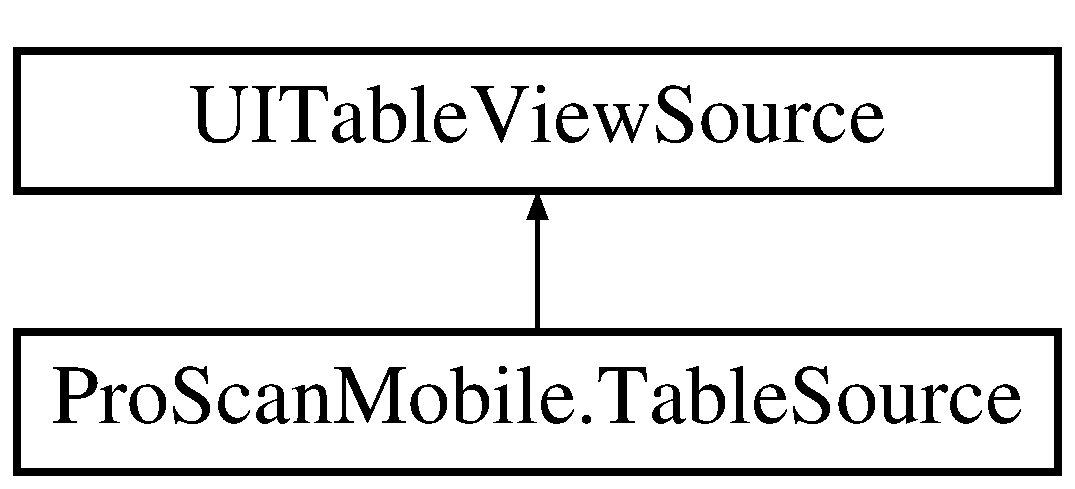
\includegraphics[height=2.000000cm]{class_pro_scan_mobile_1_1_table_source}
\end{center}
\end{figure}
\subsection*{Public Member Functions}
\begin{DoxyCompactItemize}
\item 
\hypertarget{class_pro_scan_mobile_1_1_table_source_aea9d2890a231e8bc819ef9b8989e2dcc}{{\bfseries Table\-Source} (List$<$ \hyperlink{class_pro_scan_mobile_1_1_table_item}{Table\-Item} $>$ items)}\label{class_pro_scan_mobile_1_1_table_source_aea9d2890a231e8bc819ef9b8989e2dcc}

\item 
\hypertarget{class_pro_scan_mobile_1_1_table_source_aff20e61bd340d0d4157f35da3930b646}{override float {\bfseries Get\-Height\-For\-Row} (U\-I\-Table\-View table\-View, N\-S\-Index\-Path index\-Path)}\label{class_pro_scan_mobile_1_1_table_source_aff20e61bd340d0d4157f35da3930b646}

\item 
\hypertarget{class_pro_scan_mobile_1_1_table_source_afb668953eb791c24d3d62949c38cf6dd}{override int {\bfseries Number\-Of\-Sections} (U\-I\-Table\-View table\-View)}\label{class_pro_scan_mobile_1_1_table_source_afb668953eb791c24d3d62949c38cf6dd}

\item 
\hypertarget{class_pro_scan_mobile_1_1_table_source_ade5aa9ad327a4cf7d5dc578cce50ce36}{override int {\bfseries Rows\-In\-Section} (U\-I\-Table\-View tableview, int section)}\label{class_pro_scan_mobile_1_1_table_source_ade5aa9ad327a4cf7d5dc578cce50ce36}

\item 
\hypertarget{class_pro_scan_mobile_1_1_table_source_a59cdeadc2db679679dae23b790b9f14b}{override string\mbox{[}$\,$\mbox{]} {\bfseries Section\-Index\-Titles} (U\-I\-Table\-View table\-View)}\label{class_pro_scan_mobile_1_1_table_source_a59cdeadc2db679679dae23b790b9f14b}

\item 
\hypertarget{class_pro_scan_mobile_1_1_table_source_a3105b26a6d5538b3cba5dbffd2aa11a0}{override void {\bfseries Row\-Selected} (U\-I\-Table\-View table\-View, N\-S\-Index\-Path index\-Path)}\label{class_pro_scan_mobile_1_1_table_source_a3105b26a6d5538b3cba5dbffd2aa11a0}

\item 
\hypertarget{class_pro_scan_mobile_1_1_table_source_a87cd41961f9a62200c8d198bd203e955}{override U\-I\-Table\-View\-Cell {\bfseries Get\-Cell} (U\-I\-Table\-View table\-View, Mono\-Touch.\-Foundation.\-N\-S\-Index\-Path index\-Path)}\label{class_pro_scan_mobile_1_1_table_source_a87cd41961f9a62200c8d198bd203e955}

\item 
\hypertarget{class_pro_scan_mobile_1_1_table_source_aee1a5f3bbe5f3916bdfa6b5a267b41bc}{override string {\bfseries Title\-For\-Header} (U\-I\-Table\-View table\-View, int section)}\label{class_pro_scan_mobile_1_1_table_source_aee1a5f3bbe5f3916bdfa6b5a267b41bc}

\end{DoxyCompactItemize}


\subsection{Detailed Description}


Definition at line 9 of file Table\-Source.\-cs.



The documentation for this class was generated from the following file\-:\begin{DoxyCompactItemize}
\item 
/\-Users/\-Jeff/\-Projects/\-Pro\-Scan\-Mobile+/\-Pro\-Scan\-Mobile+/\-Classes/Table\-Source.\-cs\end{DoxyCompactItemize}

\hypertarget{class_pro_scan_mobile_1_1vc_main_screen}{\section{Pro\-Scan\-Mobile.\-vc\-Main\-Screen Class Reference}
\label{class_pro_scan_mobile_1_1vc_main_screen}\index{Pro\-Scan\-Mobile.\-vc\-Main\-Screen@{Pro\-Scan\-Mobile.\-vc\-Main\-Screen}}
}
Inheritance diagram for Pro\-Scan\-Mobile.\-vc\-Main\-Screen\-:\begin{figure}[H]
\begin{center}
\leavevmode
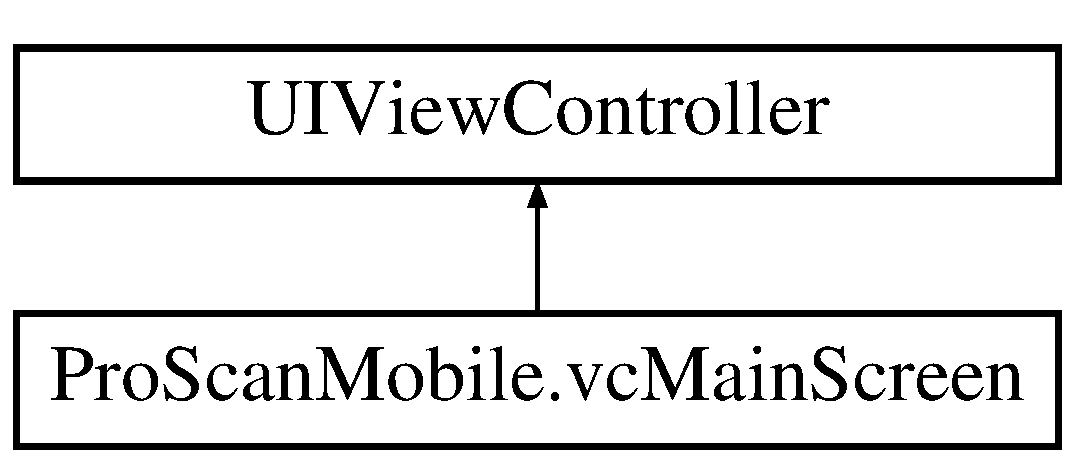
\includegraphics[height=2.000000cm]{class_pro_scan_mobile_1_1vc_main_screen}
\end{center}
\end{figure}
\subsection*{Public Member Functions}
\begin{DoxyCompactItemize}
\item 
\hypertarget{class_pro_scan_mobile_1_1vc_main_screen_a2a9f197b9f3b1459423d755cf5bc3b2c}{override void {\bfseries Did\-Receive\-Memory\-Warning} ()}\label{class_pro_scan_mobile_1_1vc_main_screen_a2a9f197b9f3b1459423d755cf5bc3b2c}

\item 
\hypertarget{class_pro_scan_mobile_1_1vc_main_screen_a2f6318f44c159832dc4cdde72714a482}{override void {\bfseries View\-Will\-Appear} (bool animated)}\label{class_pro_scan_mobile_1_1vc_main_screen_a2f6318f44c159832dc4cdde72714a482}

\item 
\hypertarget{class_pro_scan_mobile_1_1vc_main_screen_ab4ca57635214acd610e4b5934719aca2}{override void {\bfseries View\-Will\-Disappear} (bool animated)}\label{class_pro_scan_mobile_1_1vc_main_screen_ab4ca57635214acd610e4b5934719aca2}

\item 
\hypertarget{class_pro_scan_mobile_1_1vc_main_screen_addeb6f027f32ef219faaf3875da59ada}{override void {\bfseries View\-Did\-Load} ()}\label{class_pro_scan_mobile_1_1vc_main_screen_addeb6f027f32ef219faaf3875da59ada}

\end{DoxyCompactItemize}


\subsection{Detailed Description}


Definition at line 13 of file vc\-Main\-Screen.\-cs.



The documentation for this class was generated from the following files\-:\begin{DoxyCompactItemize}
\item 
/\-Users/\-Jeff/\-Projects/\-Pro\-Scan\-Mobile+/\-Pro\-Scan\-Mobile+/\-Screens/vc\-Main\-Screen.\-cs\item 
/\-Users/\-Jeff/\-Projects/\-Pro\-Scan\-Mobile+/\-Pro\-Scan\-Mobile+/\-Screens/vc\-Main\-Screen.\-designer.\-cs\end{DoxyCompactItemize}

\hypertarget{class_pro_scan_mobile_1_1vc_options_screen}{\section{Pro\-Scan\-Mobile.\-vc\-Options\-Screen Class Reference}
\label{class_pro_scan_mobile_1_1vc_options_screen}\index{Pro\-Scan\-Mobile.\-vc\-Options\-Screen@{Pro\-Scan\-Mobile.\-vc\-Options\-Screen}}
}
Inheritance diagram for Pro\-Scan\-Mobile.\-vc\-Options\-Screen\-:\begin{figure}[H]
\begin{center}
\leavevmode
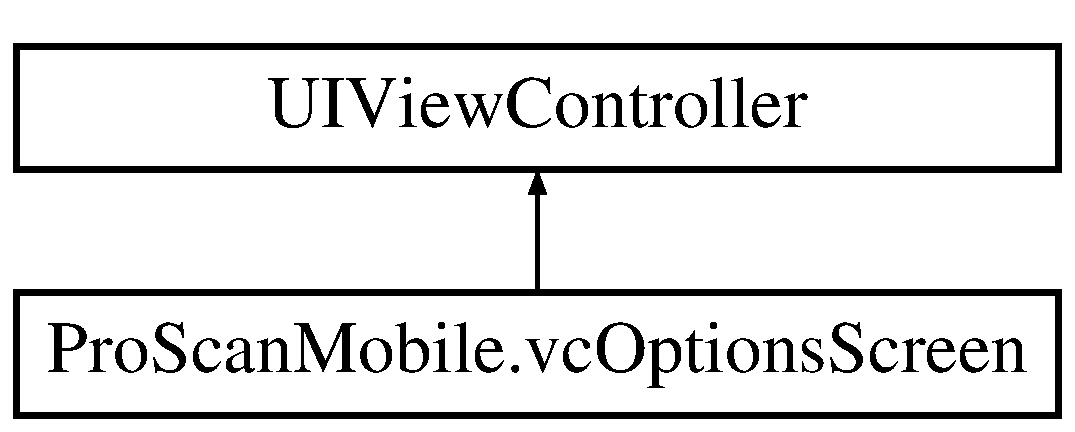
\includegraphics[height=2.000000cm]{class_pro_scan_mobile_1_1vc_options_screen}
\end{center}
\end{figure}
\subsection*{Classes}
\begin{DoxyCompactItemize}
\item 
class \hyperlink{class_pro_scan_mobile_1_1vc_options_screen_1_1_server_details}{Server\-Details}
\item 
class \hyperlink{class_pro_scan_mobile_1_1vc_options_screen_1_1_servers}{Servers}
\item 
class \hyperlink{class_pro_scan_mobile_1_1vc_options_screen_1_1_settings}{Settings}
\item 
class \hyperlink{class_pro_scan_mobile_1_1vc_options_screen_1_1_settings_details}{Settings\-Details}
\end{DoxyCompactItemize}
\subsection*{Public Member Functions}
\begin{DoxyCompactItemize}
\item 
\hypertarget{class_pro_scan_mobile_1_1vc_options_screen_a1aec538a8819aa5a3fb4b693d1548e2b}{override void {\bfseries Did\-Receive\-Memory\-Warning} ()}\label{class_pro_scan_mobile_1_1vc_options_screen_a1aec538a8819aa5a3fb4b693d1548e2b}

\item 
\hypertarget{class_pro_scan_mobile_1_1vc_options_screen_ace215be4820d6d403de4416f7e48ad77}{override void {\bfseries View\-Did\-Load} ()}\label{class_pro_scan_mobile_1_1vc_options_screen_ace215be4820d6d403de4416f7e48ad77}

\item 
\hypertarget{class_pro_scan_mobile_1_1vc_options_screen_a8aaddb5de0552580e88a1cdc2a2d080e}{override void {\bfseries View\-Will\-Appear} (bool animated)}\label{class_pro_scan_mobile_1_1vc_options_screen_a8aaddb5de0552580e88a1cdc2a2d080e}

\item 
\hypertarget{class_pro_scan_mobile_1_1vc_options_screen_a3ea1b73c4cb2c1e01ea8382a6bc27d01}{override void {\bfseries View\-Will\-Disappear} (bool animated)}\label{class_pro_scan_mobile_1_1vc_options_screen_a3ea1b73c4cb2c1e01ea8382a6bc27d01}

\item 
\hypertarget{class_pro_scan_mobile_1_1vc_options_screen_ae4ff185d2fba96c3297f4e995434044b}{void {\bfseries Get\-Settings} ()}\label{class_pro_scan_mobile_1_1vc_options_screen_ae4ff185d2fba96c3297f4e995434044b}

\item 
\hypertarget{class_pro_scan_mobile_1_1vc_options_screen_a95b59489acb4d95e6aad4555254303cd}{string {\bfseries get\-Location\-From\-Host} (string h)}\label{class_pro_scan_mobile_1_1vc_options_screen_a95b59489acb4d95e6aad4555254303cd}

\end{DoxyCompactItemize}
\subsection*{Static Public Attributes}
\begin{DoxyCompactItemize}
\item 
\hypertarget{class_pro_scan_mobile_1_1vc_options_screen_abb3cdfb902c4799355e64ea23f4c4067}{static Mono\-Touch.\-U\-I\-Kit.\-U\-I\-Text\-Field {\bfseries txt\-S\-H}}\label{class_pro_scan_mobile_1_1vc_options_screen_abb3cdfb902c4799355e64ea23f4c4067}

\item 
\hypertarget{class_pro_scan_mobile_1_1vc_options_screen_a082bba3a700d9e158b3b86add2af8599}{static Mono\-Touch.\-U\-I\-Kit.\-U\-I\-Text\-Field {\bfseries txt\-S\-P}}\label{class_pro_scan_mobile_1_1vc_options_screen_a082bba3a700d9e158b3b86add2af8599}

\item 
\hypertarget{class_pro_scan_mobile_1_1vc_options_screen_ac52f40b845e5aefde7709a6fd14365e5}{static Mono\-Touch.\-U\-I\-Kit.\-U\-I\-Text\-Field {\bfseries txt\-P\-W}}\label{class_pro_scan_mobile_1_1vc_options_screen_ac52f40b845e5aefde7709a6fd14365e5}

\end{DoxyCompactItemize}
\subsection*{Properties}
\begin{DoxyCompactItemize}
\item 
\hypertarget{class_pro_scan_mobile_1_1vc_options_screen_a90132389f95d307c2f6d1e78bbf447d9}{string {\bfseries Server\-Host\-Name}\hspace{0.3cm}{\ttfamily  \mbox{[}get\mbox{]}}}\label{class_pro_scan_mobile_1_1vc_options_screen_a90132389f95d307c2f6d1e78bbf447d9}

\item 
\hypertarget{class_pro_scan_mobile_1_1vc_options_screen_a0ec549088d412653e3c0fa2b3337fbeb}{int {\bfseries Server\-Host\-Port}\hspace{0.3cm}{\ttfamily  \mbox{[}get\mbox{]}}}\label{class_pro_scan_mobile_1_1vc_options_screen_a0ec549088d412653e3c0fa2b3337fbeb}

\item 
\hypertarget{class_pro_scan_mobile_1_1vc_options_screen_a9854fdc579de1fb2dd56d575a78b340b}{bool {\bfseries Server\-Auto\-Connect}\hspace{0.3cm}{\ttfamily  \mbox{[}get\mbox{]}}}\label{class_pro_scan_mobile_1_1vc_options_screen_a9854fdc579de1fb2dd56d575a78b340b}

\item 
\hypertarget{class_pro_scan_mobile_1_1vc_options_screen_aa2759a10f3eff93eea32706a4fd280e5}{string {\bfseries Server\-Pass\-Word}\hspace{0.3cm}{\ttfamily  \mbox{[}get\mbox{]}}}\label{class_pro_scan_mobile_1_1vc_options_screen_aa2759a10f3eff93eea32706a4fd280e5}

\end{DoxyCompactItemize}


\subsection{Detailed Description}


Definition at line 16 of file vc\-Options\-Screen.\-cs.



The documentation for this class was generated from the following files\-:\begin{DoxyCompactItemize}
\item 
/\-Users/\-Jeff/\-Projects/\-Pro\-Scan\-Mobile+/\-Pro\-Scan\-Mobile+/\-Screens/vc\-Options\-Screen.\-cs\item 
/\-Users/\-Jeff/\-Projects/\-Pro\-Scan\-Mobile+/\-Pro\-Scan\-Mobile+/\-Screens/vc\-Options\-Screen.\-designer.\-cs\end{DoxyCompactItemize}

\hypertarget{class_pro_scan_mobile_1_1vc_recordings_screen}{\section{Pro\-Scan\-Mobile.\-vc\-Recordings\-Screen Class Reference}
\label{class_pro_scan_mobile_1_1vc_recordings_screen}\index{Pro\-Scan\-Mobile.\-vc\-Recordings\-Screen@{Pro\-Scan\-Mobile.\-vc\-Recordings\-Screen}}
}
Inheritance diagram for Pro\-Scan\-Mobile.\-vc\-Recordings\-Screen\-:\begin{figure}[H]
\begin{center}
\leavevmode
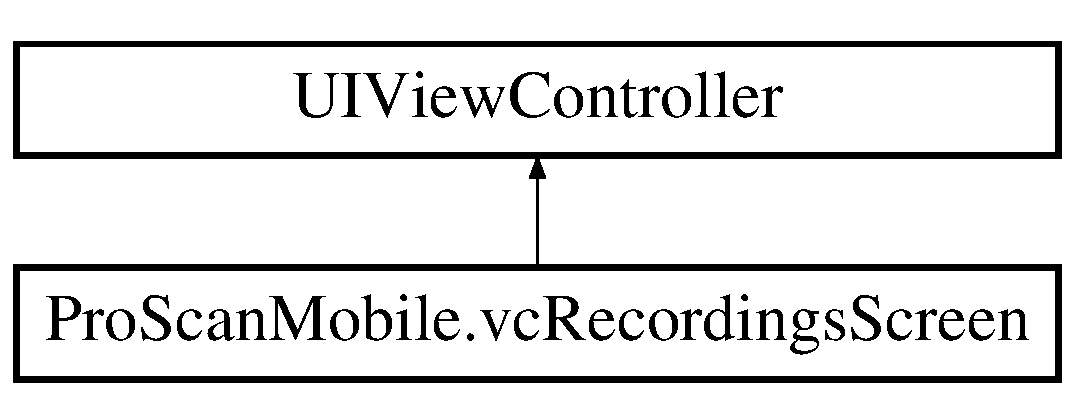
\includegraphics[height=2.000000cm]{class_pro_scan_mobile_1_1vc_recordings_screen}
\end{center}
\end{figure}
\subsection*{Public Member Functions}
\begin{DoxyCompactItemize}
\item 
\hypertarget{class_pro_scan_mobile_1_1vc_recordings_screen_a808c7d24104740d191d40d927bf41a48}{override void {\bfseries Did\-Receive\-Memory\-Warning} ()}\label{class_pro_scan_mobile_1_1vc_recordings_screen_a808c7d24104740d191d40d927bf41a48}

\item 
\hypertarget{class_pro_scan_mobile_1_1vc_recordings_screen_a4c0b51fad8f55ca86aebb07ddae4dcd6}{override void {\bfseries View\-Did\-Load} ()}\label{class_pro_scan_mobile_1_1vc_recordings_screen_a4c0b51fad8f55ca86aebb07ddae4dcd6}

\item 
\hypertarget{class_pro_scan_mobile_1_1vc_recordings_screen_a86b2e5c8fafdc097fb5a93fab2e485f8}{override void {\bfseries View\-Will\-Appear} (bool animated)}\label{class_pro_scan_mobile_1_1vc_recordings_screen_a86b2e5c8fafdc097fb5a93fab2e485f8}

\item 
\hypertarget{class_pro_scan_mobile_1_1vc_recordings_screen_a3d6b9a192bd10f5742b853197f371ece}{override void {\bfseries View\-Will\-Disappear} (bool animated)}\label{class_pro_scan_mobile_1_1vc_recordings_screen_a3d6b9a192bd10f5742b853197f371ece}

\end{DoxyCompactItemize}


\subsection{Detailed Description}


Definition at line 12 of file vc\-Recordings\-Screen.\-cs.



The documentation for this class was generated from the following files\-:\begin{DoxyCompactItemize}
\item 
/\-Users/\-Jeff/\-Projects/\-Pro\-Scan\-Mobile+/\-Pro\-Scan\-Mobile+/\-Screens/vc\-Recordings\-Screen.\-cs\item 
/\-Users/\-Jeff/\-Projects/\-Pro\-Scan\-Mobile+/\-Pro\-Scan\-Mobile+/\-Screens/vc\-Recordings\-Screen.\-designer.\-cs\end{DoxyCompactItemize}

%--- End generated contents ---

% Index
\newpage
\phantomsection
\addcontentsline{toc}{part}{Index}
\printindex

\end{document}
